% ============================================================
%  PREAMBLE - compile with XeLaTeX + biber
% ============================================================
\documentclass[12pt,a4paper]{report}

% ── Encoding & Language ──────────────────────────────────────
\usepackage{fontspec}
\setmainfont{Times New Roman}
\usepackage{polyglossia}
\setmainlanguage{english}
\usepackage{float}
% ── Page Layout ──────────────────────────────────────────────
\usepackage{geometry}
\geometry{
  a4paper,
  top=2.5cm,
  bottom=2.5cm,
  left=3cm,
  right=2.5cm
}

% ── Typography & Spacing ─────────────────────────────────────
\usepackage{setspace}
\onehalfspacing
\usepackage{parskip}
\usepackage{ragged2e}

% ── Mathematics ──────────────────────────────────────────────
\usepackage{amsmath}
\usepackage{amssymb}

% ── Graphics & Colors ────────────────────────────────────────
\usepackage{graphicx}
\usepackage{xcolor}
\usepackage{tikz}
\usetikzlibrary{positioning}

% ── Tables ───────────────────────────────────────────────────
\usepackage{array}
\usepackage{booktabs}
\usepackage{tabularx}
\usepackage{adjustbox}
\usepackage{float}

% ── Boxes & Frames ───────────────────────────────────────────
\usepackage{mdframed}

% ── Headers & Footers ────────────────────────────────────────
\usepackage{fancyhdr}

% ── Section & Chapter Formatting ─────────────────────────────
\usepackage{titlesec}
\titleformat{\chapter}[block]
  {\normalfont\Large\bfseries}{}{0em}{}
\titlespacing*{\chapter}{0pt}{0pt}{20pt}

% ── Hyperlinks (load package first) ───────────────────────────
\usepackage{hyperref}

% ── Bibliography ─────────────────────────────────────────────
\usepackage[
  backend=biber,
  style=authoryear,
  natbib=true,
  maxcitenames=2,
  uniquelist=false,
  hyperref=true,
  backref=true
]{biblatex}
\addbibresource{references.bib}

% ── Hyperlink config (after biblatex to prevent settings reset)
\hypersetup{
  colorlinks=true,
  linkcolor=blue,
  citecolor=blue,
  urlcolor=blue,
  pdfborder={0 0 0},
  hyperindex=true,
  pageanchor=true,
  linktoc=all
}

% ── Make the ENTIRE citation (author + year) clickable ───────
\DeclareCiteCommand{\cite}
  {\usebibmacro{prenote}}
  {\usebibmacro{citeindex}%
   \printtext[bibhyperref]{\usebibmacro{cite}}}
  {\multicitedelim}
  {\usebibmacro{postnote}}

\DeclareCiteCommand{\parencite}[\mkbibparens]
  {\usebibmacro{prenote}}
  {\usebibmacro{citeindex}%
   \printtext[bibhyperref]{\usebibmacro{cite}}}
  {\multicitedelim}
  {\usebibmacro{postnote}}

\DeclareCiteCommand{\textcite}
  {\boolfalse{cbx:parens}}
  {\usebibmacro{citeindex}%
   \printtext[bibhyperref]{\usebibmacro{textcite}}}
  {\ifbool{cbx:parens}
     {\bibcloseparen\global\boolfalse{cbx:parens}}
     {}%
   \multicitedelim}
  {\usebibmacro{textcite:postnote}}

\DeclareCiteCommand{\citet}
  {\boolfalse{cbx:parens}}
  {\usebibmacro{citeindex}%
   \printtext[bibhyperref]{\usebibmacro{textcite}}}
  {\ifbool{cbx:parens}
     {\bibcloseparen\global\boolfalse{cbx:parens}}
     {}%
   \multicitedelim}
  {\usebibmacro{textcite:postnote}}

\DeclareCiteCommand{\citep}[\mkbibparens]
  {\usebibmacro{prenote}}
  {\usebibmacro{citeindex}%
   \printtext[bibhyperref]{\usebibmacro{cite}}}
  {\multicitedelim}
  {\usebibmacro{postnote}}

% ============================================================
\usepackage{placeins}

% ── Arabic support (must be loaded last for bidi) ────────────
\newfontfamily\arabicfont[Script=Arabic]{Amiri}
\setotherlanguage{arabic}

% ── Page numbers everywhere (arabic style with fancyhdr) ─────
\pagestyle{fancy}
\fancyhf{}
\fancyhead[R]{\thepage}
\fancyhead[L]{\nouppercase{\leftmark}}
\renewcommand{\headrulewidth}{0.4pt}

\begin{document}

% ── FRONT MATTER (roman page numbers) ───────────────────────
\pagestyle{empty}
\pagenumbering{roman}


% ============================================================
%  PAGE 1 - COVER PAGE  (single page, as required)
% ============================================================
\begin{titlepage}
\vspace*{-1.2cm}  % reduce top margin further

% Page double border
\begin{tikzpicture}[remember picture, overlay]
  \draw[line width=2pt]
    ([shift={(0.55cm,0.55cm)}]current page.south west)
    rectangle
    ([shift={(-0.55cm,-0.55cm)}]current page.north east);
  \draw[line width=0.5pt]
    ([shift={(0.7cm,0.7cm)}]current page.south west)
    rectangle
    ([shift={(-0.7cm,-0.7cm)}]current page.north east);
\end{tikzpicture}

% Watermark
\begin{tikzpicture}[remember picture, overlay]
  \node[opacity=0.07] at (current page.center)
    {
\includegraphics[width=0.68\paperwidth]{picture/logo/logo.png}};
\end{tikzpicture}

% ── Arabic header ───────────────────────────────────────
\begin{center}
  {\small\bfseries People's Democratic Republic of Algeria}\\[0.5pt]
  {\small\bfseries Ministry of Higher Education and Scientific Research}
\end{center}

\vspace{1pt}
\noindent\rule{\linewidth}{0.5pt}
\vspace{1pt}

% ── University row ──────────────────────────────────────
\begin{center}
\begin{tabular}{p{0.34\linewidth} c p{0.34\linewidth}}
  \raggedright
  {\footnotesize Universit\'e Badji Mokhtar -- Annaba\\
           Badji Mokhtar -- Annaba University} &
  \raisebox{-0.4cm}{%
    
\includegraphics[height=1.5cm]{picture/logo/logo.png}} &
  \raggedleft
  {\footnotesize\bfseries Universit\'e Badji Mokhtar\\
                   -- Annaba --}
\end{tabular}
\end{center}

\vspace{1pt}
\noindent\rule{\linewidth}{0.5pt}
\vspace{1pt}

% ── Faculty block (more compact) ────────────────────────
\begin{flushleft}
  {\footnotesize \textbf{Faculty:} Technology}\\[0.5pt]
  {\footnotesize \textbf{Department:} Computer Science}\\[0.5pt]
  {\footnotesize \textbf{Domain:} Mathematics -- Computer Science}\\[0.5pt]
  {\footnotesize \textbf{Field:} Computer Science}\\[0.5pt]
  {\footnotesize \textbf{Speciality:} Information Systems and Decision Support}
\end{flushleft}

\vspace{0.1cm}

% ── Memoir label ────────────────────────────────────────
\begin{center}
  {\large\bfseries Memoir}\\[1pt]
  {\normalsize Presented for the award of the \textbf{Master's Degree}}
\end{center}

\vspace{0.05cm}
\begin{center}{\large\bfseries Theme}\end{center}
\vspace{0.05cm}

% ── Title box (more compact) ────────────────────────────
\begin{mdframed}[
  linecolor=black, linewidth=1pt,
  innertopmargin=4pt, innerbottommargin=4pt,
  innerleftmargin=8pt, innerrightmargin=8pt,
  roundcorner=4pt
]
  \begin{center}
    {\bfseries
      Leveraging Deep Learning Techniques for Advanced\\[2pt]
      Recommender Systems
    }
  \end{center}
\end{mdframed}

\vspace{0.2cm}

% ── Author ──────────────────────────────────────────────
\begin{center}
  \textbf{Presented by:} \quad Farouk Ouled Meriem
\end{center}

\vspace{0.15cm}

% ── Supervisor ──────────────────────────────────────────
\begin{center}
  \begin{tabular}{lll}
    \textbf{Supervisor:} & Samira Lagrini \quad & MCA \quad Badji Mokhtar -- Annaba University
  \end{tabular}
\end{center}

\vspace{0.15cm}

% ── Jury table (even more compact) ──────────────────────
\begin{center}
  \textbf{Defense Jury:}\\[2pt]
  {\footnotesize
  \renewcommand{\arraystretch}{0.7}
  \begin{tabular}{|p{3.4cm}|p{1.3cm}|p{3.8cm}|p{2.0cm}|}
    \hline
    Zenati Soraya     & MCB & Badji Mokhtar -- Annaba University & President   \\ \hline
    Lagrini Samira    & MCA & Badji Mokhtar -- Annaba University & Supervisor  \\ \hline
    Yakoubi Med Amine & MCA & Badji Mokhtar -- Annaba University & Examiner    \\ \hline
  \end{tabular}
  }
\end{center}

\vfill  % pushes year to bottom of same page

\begin{center}
  {\normalsize\bfseries University Year: 2025/2026}
\end{center}

\end{titlepage}



% ============================================================
%  PAGE 2 - ACKNOWLEDGEMENTS
% ============================================================
\newpage
% Activate page numbering for front matter
\pagestyle{fancy}
\chapter*{Acknowledgements}
\addcontentsline{toc}{chapter}{Acknowledgements}

\begin{center}
\textbf{In the name of Allah, the Most Gracious, the Most Merciful.}
\end{center}

First and foremost, all praise and gratitude are due to \textbf{Allah}, who
gave me the strength, patience, and perseverance to complete this work. Without
His will and guidance, nothing would have been possible. \textbf{Alhamdulillah.}

\vspace{0.5cm}

\noindent\textbf{\large To my beloved parents,}

\textbf{My mother} -- your unconditional love, your tenderness, and your
prayers have carried me and protected me in every moment of doubt. You are the
gentle light that guides my steps, even when the path is dark. Your faith in me
has so often been stronger than my own. Thank you for everything.

\textbf{My father} -- your patience, your wisdom, and your quiet strength have
been my foundation. Through your proud gaze and your reassuring silence, you
taught me perseverance, dignity, and respect. You are my pillar, my compass,
my root.

This thesis is far more than an academic achievement: it is the fruit of your
love, your sacrifices, and your constant presence. Thank you for all that you
have given me, and for all that you are.

\vspace{0.5cm}

\noindent\textbf{\large To my siblings}

\textbf{Abdel El Kader}, \textbf{Seif El Islam Deneche}, and
\textbf{Nour El Houda} -- your simple but powerful words, your sincere smiles,
and your calming presence have meant the world to me. Thank you for being there
without needing to speak, and for always supporting me.

\vspace{0.5cm}

\noindent\textbf{\large To my true friends}

Thank you for your kind words, your caring silences, your spontaneous laughter,
and your positive energy. Your friendship has been a precious gift.

\vspace{0.5cm}

\noindent\textbf{\large To my supervisor, Madame Samira Lagrini}

Thank you for your thoughtful guidance, your wise advice, and your trust in me.
Thanks to you, I have grown both intellectually and personally. Your support
has been invaluable.

\vspace{0.5cm}

\noindent\textbf{\large To my SID Master's cohort (2024--2026)}

Thank you for the journey we have walked together -- shared efforts, mutual
support, and lasting memories. You have been far more than classmates; you have
been true companions on this academic adventure. I am grateful for your
kindness, your smiles, and your team spirit. This thesis also reflects these
unforgettable years.

\vspace{0.5cm}

\noindent\textbf{\large To the members of the jury}

I wish to express my sincere gratitude for the honour you have given me by
taking the time to read and evaluate this work.

\vspace{1cm}

\begin{center}
To all those who are dear to me, thank you. This thesis, signed by my hand,
also carries the imprint of each of you.
\end{center}


% ============================================================
%  PAGE 3 - DEDICATIONS
% ============================================================
\newpage
\chapter*{Dedications}
\addcontentsline{toc}{chapter}{Dedications}

\vspace{2.5cm}

\begin{center}
  \itshape\large
  To my parents,\\[8pt]
  for every sacrifice they made so I could reach this day.\\[24pt]

  To my family and friends,\\[8pt]
  for their constant support and encouragement.\\[24pt]

  \upshape\normalsize\textbf{Farouk Ouled Meriem}
\end{center}


% ============================================================
%  TABLE OF CONTENTS, LIST OF FIGURES, LIST OF TABLES
% ============================================================
\newpage
\tableofcontents
\newpage
\listoffigures
\newpage
\listoftables


% ============================================================
%  GENERAL INTRODUCTION (Unnumbered Chapter)
% ============================================================
\newpage
\pagenumbering{arabic}

\chapter*{General Introduction}
\addcontentsline{toc}{chapter}{General Introduction}

% ── Context and Motivation ───────────────────────────────────
\section*{Context and Motivation}

\justifying
The era of digital transformation has connected millions of users through
online platforms that have become central to daily life. E-commerce sites
allow people to purchase and sell products worldwide, while streaming
services such as YouTube provide instant access to entertainment including
films, music, and video content.
The rapid developments in the digital domain have produced an exponential
growth in the volume of online content. Such an abundance of choices makes
it increasingly difficult for users to locate relevant content aligned with
their interests, and can impair or paralyse the decision-making process.
Recommendation systems were developed specifically to address this challenge.
By learning user interests and behavioral patterns, they help users discover
products, services, or content they are likely to enjoy.
Recommendation systems span several categories; sequential recommendation
is one of the most active research directions in recent years. Unlike
classical collaborative filtering approaches, which identify user interests
through group similarities, sequential recommendation models exploit the
temporal order of user interaction histories to predict the next item a
user is likely to engage with -- whether through purchase, viewing, or
listening. By capturing the ordered sequence of past behaviors, these models
better track dynamic user interests and provide more timely recommendations.

Deep learning has been a major driving force in sequential recommendation.
Among early contributions, \citet{hidasi2016gru4rec} showed that gated
recurrent networks are effective at capturing session-level dynamics for
next-item prediction. Attention mechanisms and Transformer-based architectures
later provided a substantial leap forward: models such as SASRec
\citep{kang2018sasrec} and BERT4Rec \citep{sun2019bert4rec} demonstrated
that learning dependencies across entire interaction sequences yields better
accuracy and scalability than recurrent approaches.
Graph Neural Networks were subsequently introduced to model the global
relational structure among users and items, extracting collaborative
information that purely sequential models cannot access.

However, these two paradigms have complementary strengths and weaknesses.
Graph Neural Networks excel at capturing global item co-occurrence patterns
but are limited in modeling the fine-grained temporal context within a
user's history. Sequence-based Transformer models are strong at encoding
recent user preferences but cannot leverage information beyond an individual
user's own interactions. Existing hybrid approaches generally combine these
two components using a fixed, user-agnostic fusion weight. Yet users differ
substantially in how much interaction history they have accumulated, and the
relative reliability of the graph signal versus the sequential signal
varies accordingly. Users with sparse histories benefit more from global
collaborative information, while users with rich histories can better
exploit detailed sequential patterns.

At the same time, Large Language Models (LLMs) such as GPT, LLaMA, and
BERT, pre-trained on large text corpora, have demonstrated a remarkable
capacity to encode semantic knowledge about items and contexts
\citep{wu2023survey,liu2024llmers}. Their integration into recommendation
systems has opened a new direction: using LLM-derived embeddings to
enrich item representations with semantic information that interaction
data alone cannot provide \citep{harte2023leveraging,llmrec2024}. However,
a fundamental question remains underexplored: how should the textual
description of an item be constructed in order to maximally leverage the
semantic content captured by LLM embeddings in a sequential recommendation
setting? Different description strategies produce embeddings with different
properties, which may significantly influence downstream recommendation
quality.

% ── Addressed Research Problems ──────────────────────────────
\section*{Addressed Research Problems}

This memoir addresses two complementary research problems:

\medskip
\noindent\textbf{Problematic 1} - \textit{How to dynamically adapt the
fusion between global graph signals and local sequential modelling according
to each user's interaction history profile?}

\medskip
\noindent\textbf{Problematic 2} - \textit{How does the choice of item
textual description strategy influence the quality of LLM embeddings in
sequential recommendation?}

% ── Main Contributions ───────────────────────────────────────
\section*{Main Contributions}

This work presents two main contributions:

\begin{itemize}
  \item \textbf{Contribution 1}: A hybrid GNN-Transformer model with adaptive
  fusion based on user interaction history length.
  \item \textbf{Contribution 2}: A systematic study of the impact of item
  description strategies on LLM embedding quality for sequential
  recommendation.
\end{itemize}

% ── Memoir Organization ──────────────────────────────────────
\section*{Memoir Organization}

The rest of this memoir is structured as follows:

\medskip
\textbf{Chapter 1} describes the basic concepts and the state-of-the-art
methods for sequential recommendation systems. It covers classical approaches,
sequence-based and graph-based deep learning models, Large Language Models, and
evaluation criteria. It ends with the research gaps that motivated this work.

\textbf{Chapter 2} proposes our first contribution: a Length-Adaptive Hybrid
GNN-Transformer. It describes the shortcomings of previous models, formalizes
the problem, and provides the details of the proposed architecture and fusion
method.

\textbf{Chapter 3} illustrates the experiments of the first contribution. It
contains the description of datasets, pre-processing, baselines, parameters,
experimental results, and an ablation study.

\textbf{Chapter 4} discusses the second contribution: a comprehensive analysis
of item description strategies for LLM-based sequential recommendation. It
presents the \texttt{LLM2Sequential} pipeline and seven description strategies
proposed in this work.

\textbf{Chapter 5} presents the evaluation experiments of the second
contribution and compares all the strategies against a previous work
\citep{boz2025}.

Lastly, a \textbf{General Conclusion} presents the main findings, the
limitations, and future research directions.


% ============================================================
%  CHAPTER 1 - Foundations and State of the Art
% ============================================================
\chapter{Foundations and State of the Art}

\section{Introduction to Recommendation Systems}

\justifying
Recommendation systems (RS) are methods for filtering large volumes of data
and surfacing items that match a given user's tastes and interests
\citep{castells2023primer}. As digital catalogs grow -- from product
listings on e-commerce platforms to the libraries of streaming services --
the volume of available choices has outpaced users' capacity to evaluate
them individually, creating what the literature commonly refers to as the
information overload problem \citep{raza2024comprehensive}. The goal of RS
is to identify item patterns according to item characteristics and user
interest profiles so as to recommend relevant content by analysing
behavioral signals. Recommendation systems have become core infrastructure
in modern intelligent applications across domains including e-commerce,
media, and music \citep{raza2024comprehensive}.

There are three common paradigms used to develop a recommendation system, as
illustrated in Figure~\ref{fig:rs_taxonomy}:

\begin{itemize}
    \item \textbf{Collaborative Filtering (CF):} Recommends items by
    leveraging the past behavior of users, on the assumption that users who
    agreed in the past will continue to agree in the future. CF can either
    use the interaction data itself (memory-based) or latent factor models
    learnt from the data (model-based) \citep{castells2023primer}.

    \item \textbf{Content-Based Filtering (CB):} Recommends items with the
    same characteristics as the ones the user previously showed affinity for,
    by comparing item features with an individual user profile
    \citep{raza2024comprehensive}.

    \item \textbf{Hybrid Systems:} Combinations of CF and CB methods are often
    developed in order to overcome the drawbacks of both methods -- for
    example cold-start in CF and over-specialization in CB -- and therefore
    build more efficient recommendation systems \citep{raza2024comprehensive}.
\end{itemize}

\begin{figure}[htbp]
    \centering
    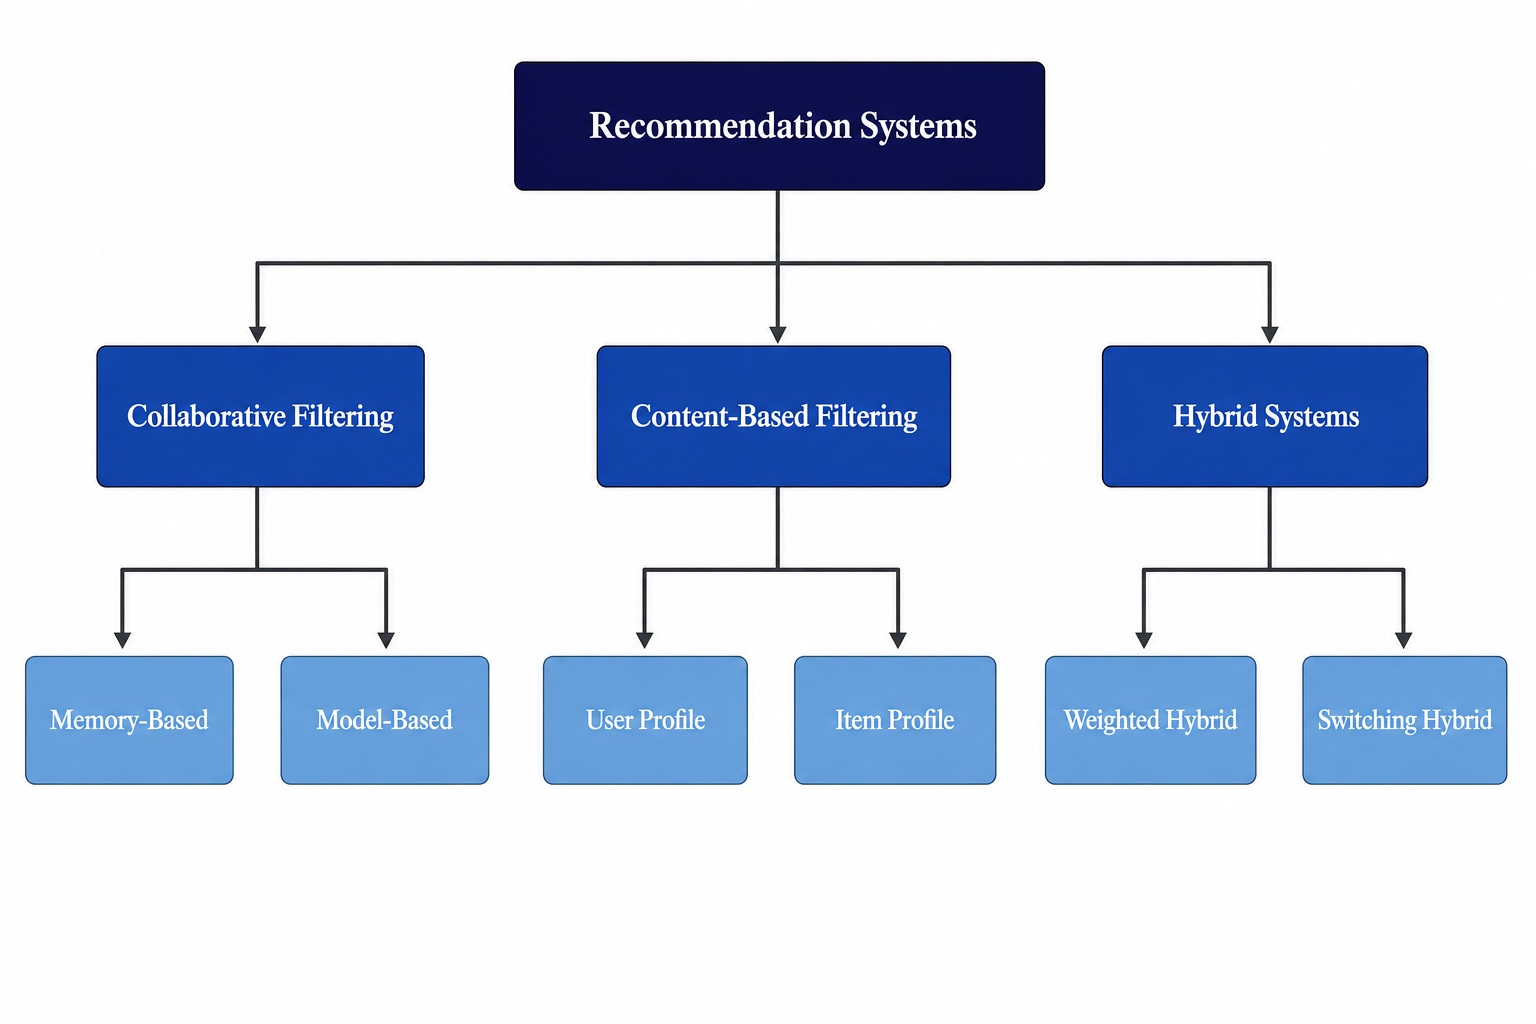
\includegraphics[width=0.95\textwidth]{picture/figures/schemas/taxonomy_reco.png}
    % CORRECTION: shortened caption to one explicit line
    \caption{Taxonomy of recommendation system types.}
    \label{fig:rs_taxonomy}
\end{figure}

Out of the above, sequential recommendation systems form a subcategory and have
gradually become a more and more important area of collaborative filtering,
where the order in which users interacted with items is considered. This work
concentrates only on this type of systems. Formally they are defined below.

\section{Sequential Recommendation}

\justifying
In sequential recommendation (SR), the task of predicting the next item to recommend to a user depends not only on the set of items with which the user has interacted, but also on the specific order of these interactions \citep{pan2024survey}. This sequence is important, as users' preferences are dynamic: short-term preferences often have higher weight than long-term ones and the meaning of the action is interpreted differently based on the context that precedes it (for example, clicking an item does not carry the same semantics as purchasing it). SR is typically framed as the task of predicting the next item given a sequence of past interactions and is naturally suited for scenarios where dynamic, short-term intent needs to be modeled, such as e-commerce, news recommendation, or media streaming \citep{hidasi2016gru4rec,kang2018sasrec,sun2019bert4rec}.

Deep learning has led to major advances in the area of SR, due to models that are able to incorporate sequential dependencies explicitly. Among the early ones, the use of gated recurrent networks such as GRU4Rec was shown to be effective in capturing session-level dynamics and improving next-item prediction \citep{hidasi2016gru4rec}. Self-attention based models, like SASRec, proposed an effective solution to model dependencies across full interaction sequences \citep{kang2018sasrec}, and then BERT4Rec utilized bidirectional context through a masked item prediction objective \citep{sun2019bert4rec}. These papers have consolidated SR as a major research direction in recommender systems.

In practice, SR remains challenging because interaction sequences can be very sparse, short, long, or heterogeneous, which complicates accurate modeling. Short sequences contain little evidence about user preferences, while long sequences may include irrelevant interactions that dilute the user's current intent. Moreover, variable time gaps between interactions and differing action semantics increase the difficulty of balancing short-term and long-term interests. Consequently, recent work emphasizes more powerful sequence encoders, hybrid architectures that combine global and local signals, incorporation of side information, and integration with large language models to improve robustness and representation quality \citep{pan2024survey}.

\begin{figure}[htbp]
    \centering
    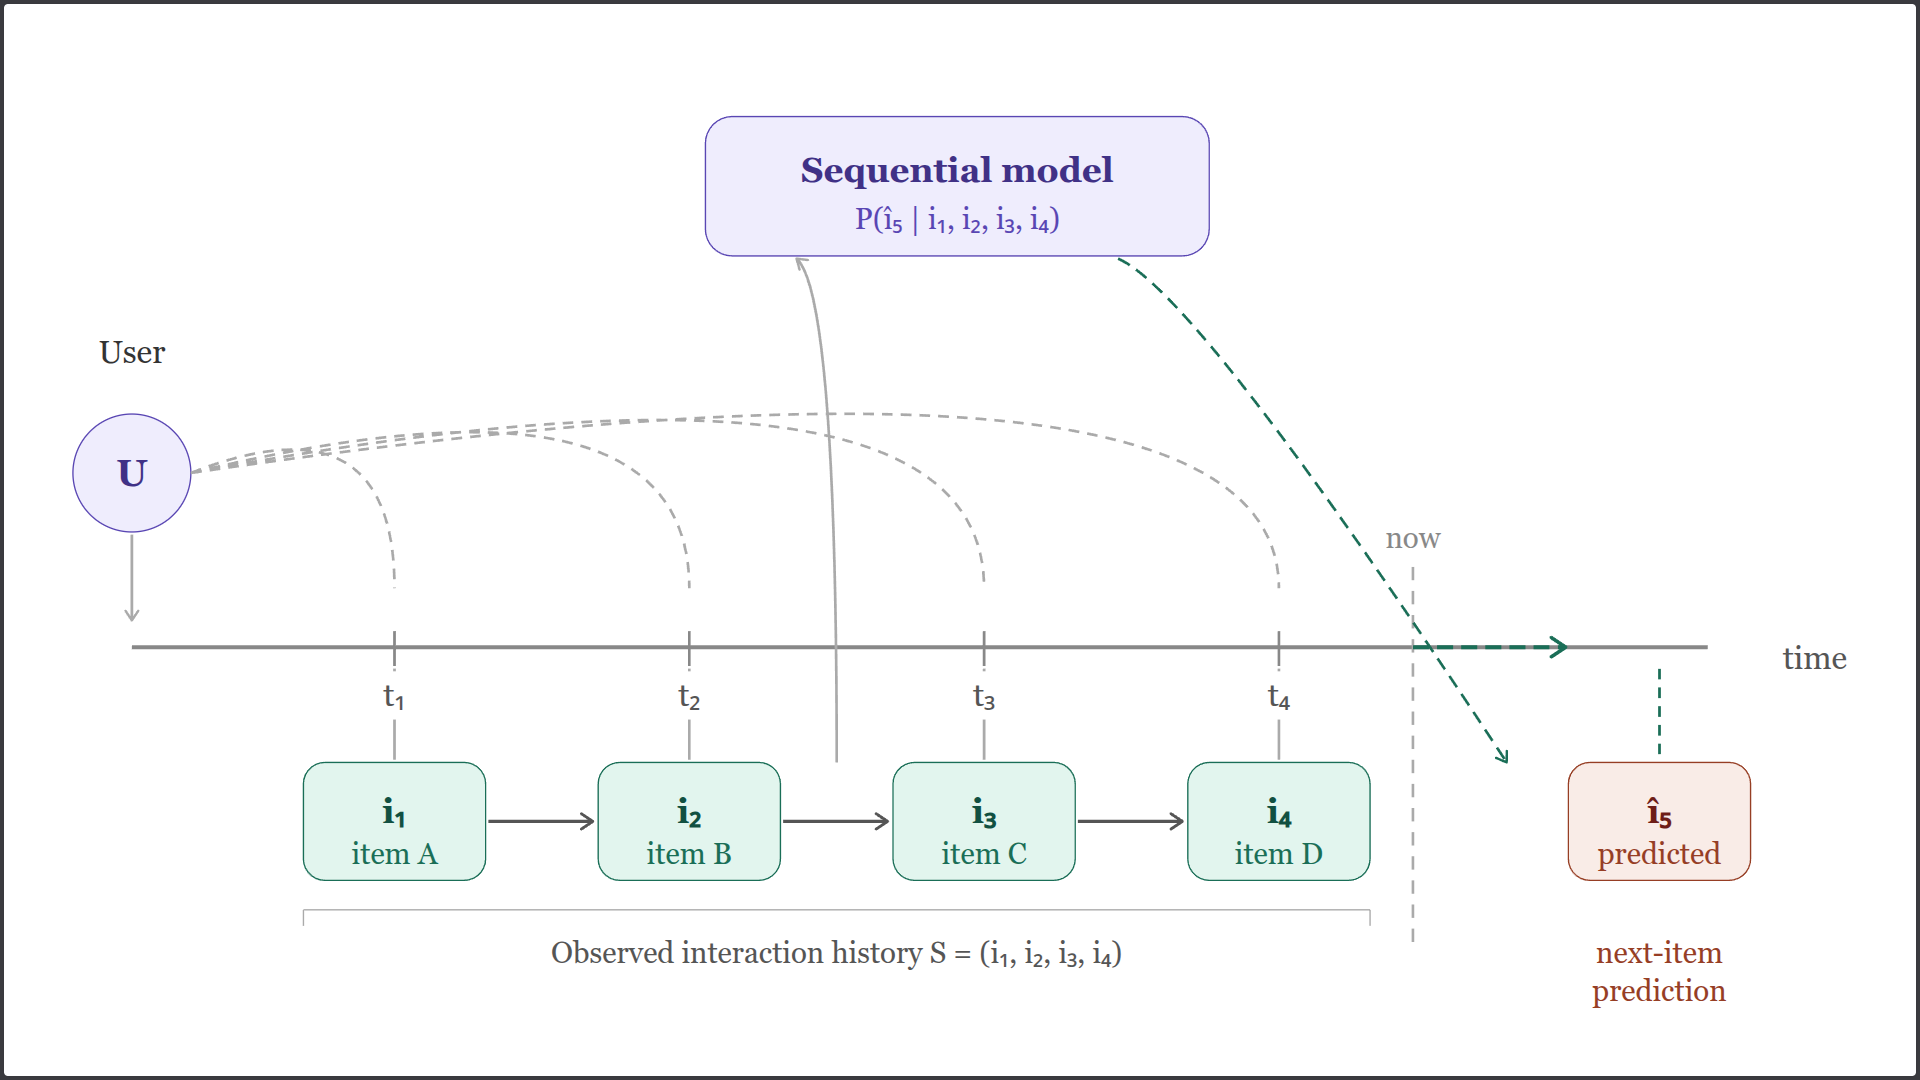
\includegraphics[
        width=0.9\textwidth,
        trim=20 20 20 20,
        clip
    ]{picture/figures/schemas/sequential_recommendation_timeline.png}
    % CORRECTION: shortened caption to one explicit line
    \caption{User interaction timeline for sequential next-item prediction.}
    \label{fig:sequential_timeline}
\end{figure}

\section{Sequence-Based Models}

\justifying
Sequence-based models constitute an important class of sequential recommendation
methods that explicitly exploit the ordered nature of user interaction histories.
Unlike simpler approaches that treat a user's past actions as an unordered set,
these models learn patterns from the exact sequence of events in order to
predict the next likely item. This family of methods formed one of the earliest
and most influential directions in sequential recommendation, and it includes
recurrent, convolutional, and Transformer-based architectures.

\subsection{GRU4Rec}

\justifying
GRU4Rec was one of the first deep learning models proposed for session-based
recommendation and showed that recurrent neural networks can effectively model
sequential user behavior \citep{hidasi2016gru4rec}. The model uses gated
recurrent units to process interaction sequences in order, allowing it to
capture short-term dependencies and session-level dynamics. Its key idea is that
the hidden state summarizes the recent behavior of the user, which is then used
to predict the next item in the sequence. This made GRU4Rec an important
baseline for later sequential recommendation research.

\subsection{Caser}

\justifying
Caser introduces a convolutional approach to sequential recommendation by
embedding a user's recent interaction history into a two-dimensional
representation and applying convolutional filters over it \citep{tang2018caser}.
The model is designed to capture both general user preferences and local
sequential patterns through vertical and horizontal convolutions. In contrast to
recurrent models, Caser views the sequence as a structured pattern detection
problem, which allows it to learn influential subsequences and short-range
dependencies. This makes Caser a representative CNN-based baseline in the SR
literature.

\subsection{SASRec}

\justifying
SASRec applies self-attention to sequential recommendation, using a
Transformer-style architecture to model dependencies between interacted items
across the full interaction history \citep{kang2018sasrec}. Instead of
processing the sequence strictly step by step, the model learns which past items
are most relevant to the current prediction through attention weights. This gives
SASRec a strong ability to capture both short- and long-term behavioral patterns
while remaining efficient to train. It became one of the most influential
Transformer-based baselines in sequential recommendation.

\subsection{BERT4Rec}

\justifying
BERT4Rec extends the Transformer idea by adopting a bidirectional encoding
strategy and a masked item prediction objective \citep{sun2019bert4rec}. Rather
than predicting the next item in a strictly left-to-right fashion, the model
randomly masks items in the sequence and learns to reconstruct them from both
left and right context. This training objective encourages richer sequence
representations and often improves the quality of learned user behavior
embeddings. BERT4Rec is widely used as a strong benchmark for sequential
recommendation due to its ability to model contextual dependencies more deeply.

\begin{figure}[htbp]
    \centering
    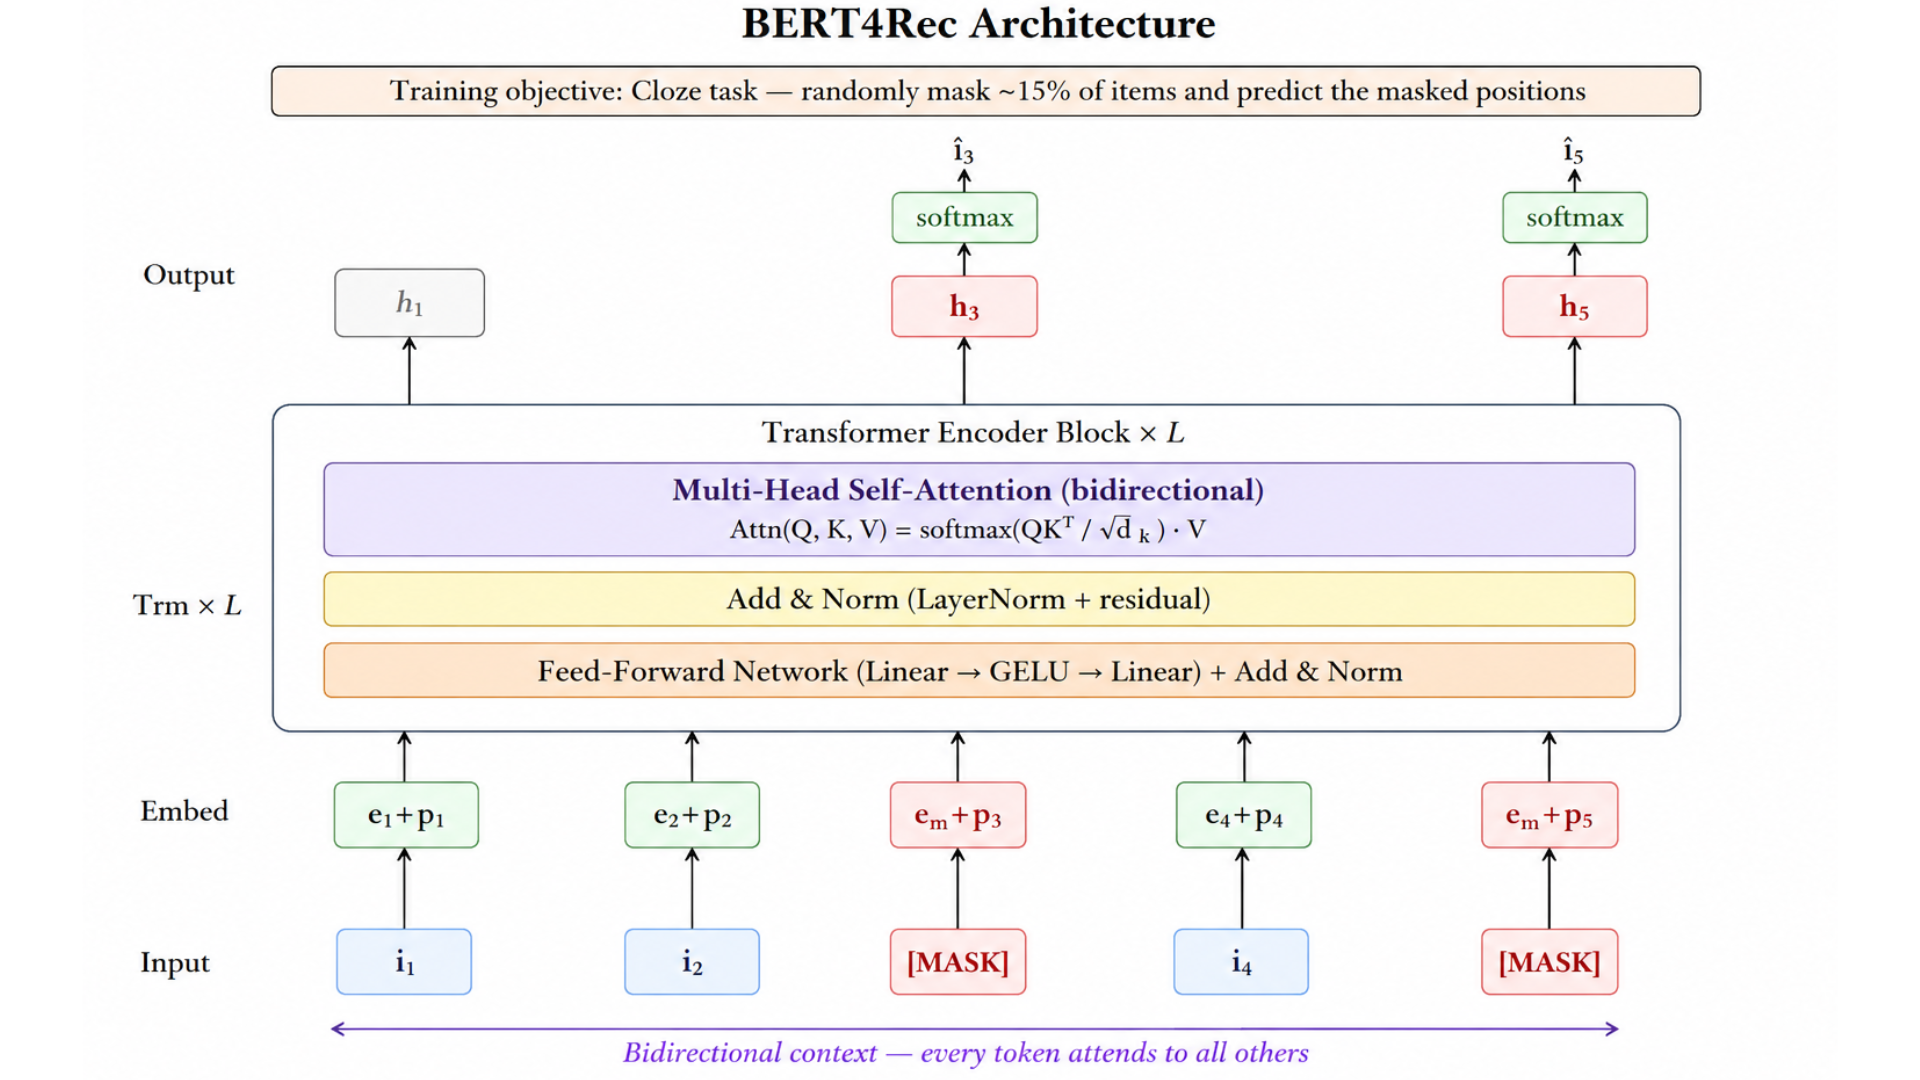
\includegraphics[width=0.9\textwidth]{picture/figures/schemas/bert4rec_architecture.png}
    % CORRECTION: shortened caption to one explicit line
    \caption{Architecture of a Transformer-based sequential model (SASRec/BERT4Rec).}
    \label{fig:sequence_architecture}
\end{figure}

\begin{table}[h]
\centering
\begin{tabular}{p{2.4cm} p{3.3cm} p{7.0cm}}
\toprule
\textbf{Model} & \textbf{Approach} & \textbf{Key idea} \\
\midrule
GRU4Rec & Recurrent neural network & Models the interaction sequence step by step with gated recurrent units. \\
Caser & Convolutional neural network & Learns local sequential patterns from a sequence-as-image representation. \\
SASRec & Self-attention / Transformer encoder & Uses attention to focus on the most relevant past items for next-item prediction. \\
BERT4Rec & Bidirectional Transformer encoder & Learns contextual sequence representations using masked item prediction. \\
\bottomrule
\end{tabular}
% CORRECTION: shortened table caption to one explicit line
\caption{Representative sequence-based recommendation models.}
\label{tab:sequence_models}
\end{table}

\section{Graph-Based Models / GNN}

\justifying
Graph-based recommender systems model user-item interactions as a graph, where
users and items are represented as nodes and historical interactions are encoded
as edges. This formulation is useful because recommendation data are naturally
relational: a user's preference can be inferred not only from their own history,
but also from their position in the interaction graph and from the neighborhoods
of connected users and items. Graph neural networks therefore provide a powerful
way to propagate collaborative signals, capture higher-order connectivity, and
learn richer embeddings than methods based solely on local sequence patterns
\citep{wu2020gnnsurvey,he2020lightgcn}.

\subsection{LightGCN}

\justifying
LightGCN is one of the most influential graph-based recommendation models
because it simplifies graph convolution to its essential component:
neighborhood aggregation \citep{he2020lightgcn}. Instead of using feature
transformation and nonlinear activation, LightGCN directly propagates user and
item embeddings over the bipartite interaction graph and combines the embeddings
from multiple propagation layers to obtain the final representation. This makes
the model both efficient and effective, and it has become a standard baseline
for graph-based collaborative filtering. Its main strength is the ability to
capture collaborative signals from the full interaction graph while remaining
simple enough to train and interpret.

\begin{table}[h]
\centering
\begin{tabular}{p{3cm} p{3cm} p{6.8cm}}
\toprule
\textbf{Model} & \textbf{Approach} & \textbf{Key idea} \\
\midrule
LightGCN & Graph collaborative filtering & Learns user and item embeddings by propagating them over the bipartite interaction graph with only neighborhood aggregation. \\
\bottomrule
\end{tabular}
% CORRECTION: shortened table caption to one explicit line
\caption{Representative graph-based recommendation models.}
\label{tab:graph_models}
\end{table}

\begin{figure}[htbp]
    \centering
    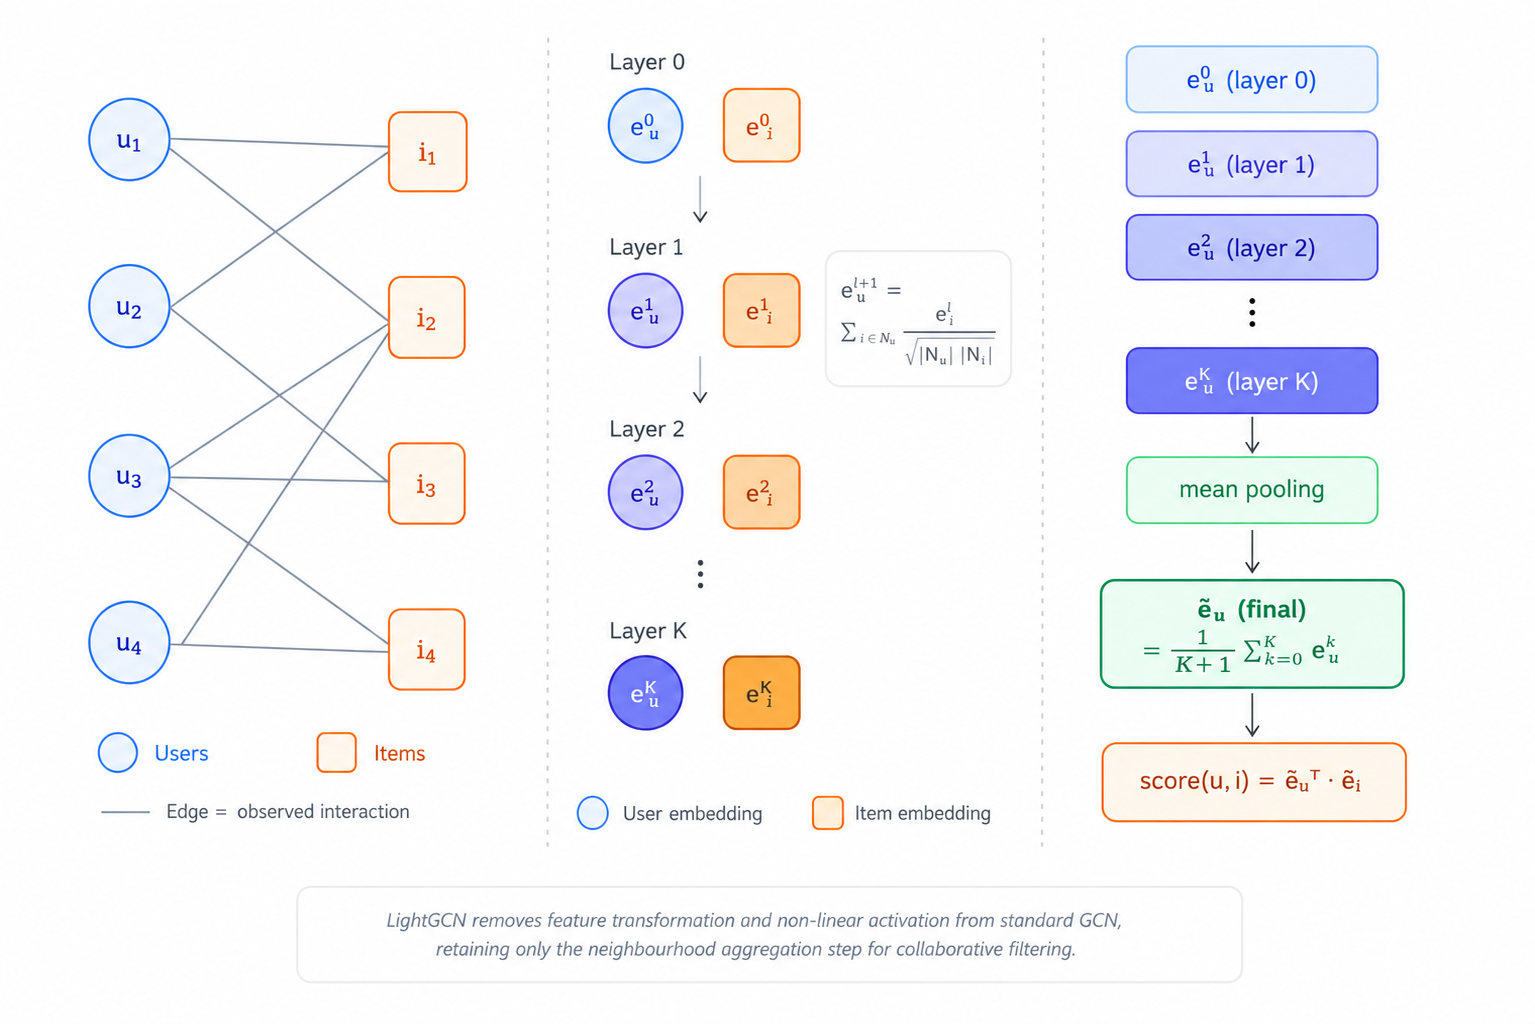
\includegraphics[width=0.9\textwidth]{picture/figures/schemas/lightgcn_bipartite_graph.png}
    % CORRECTION: shortened caption to one explicit line
    \caption{Bipartite user-item graph and embedding propagation in LightGCN.}
    \label{fig:lightgcn_graph}
\end{figure}

\section{LLMs Applied to Sequential Recommendation}

\justifying
Large Language Models (LLMs) have recently entered recommendation systems by
bringing strong semantic understanding of text, contextual reasoning, and
transferable representations learned from large-scale corpora. In sequential
recommendation, this is particularly valuable because many items are described
by textual metadata such as titles, descriptions, reviews, or categorical
attributes. Rather than relying only on item identifiers or interaction history,
LLM-based methods can transform item text into dense embeddings that encode
semantic similarity and can be injected into recommendation pipelines as
initialization, side information, or direct ranking signals
\citep{harte2023leveraging,llmrec2024,wu2023survey,liu2024llmers}.

A central idea in this line of work is that the textual description of an item
can act as a semantic bridge between sparse interaction data and richer domain
knowledge. When item descriptions are encoded by an LLM, the resulting
embeddings can capture not only surface-level wording, but also relations
between concepts, product properties, and user-facing meaning. These embeddings
can then be used to improve sequential recommenders by initializing item
representations, enhancing content-based signals, or supporting hybrid models
that combine textual and behavioral information. This is especially helpful in
cold-start or sparse-data settings, where item IDs alone provide little
information about the item's semantics.

\begin{figure}[htbp]
    \centering
    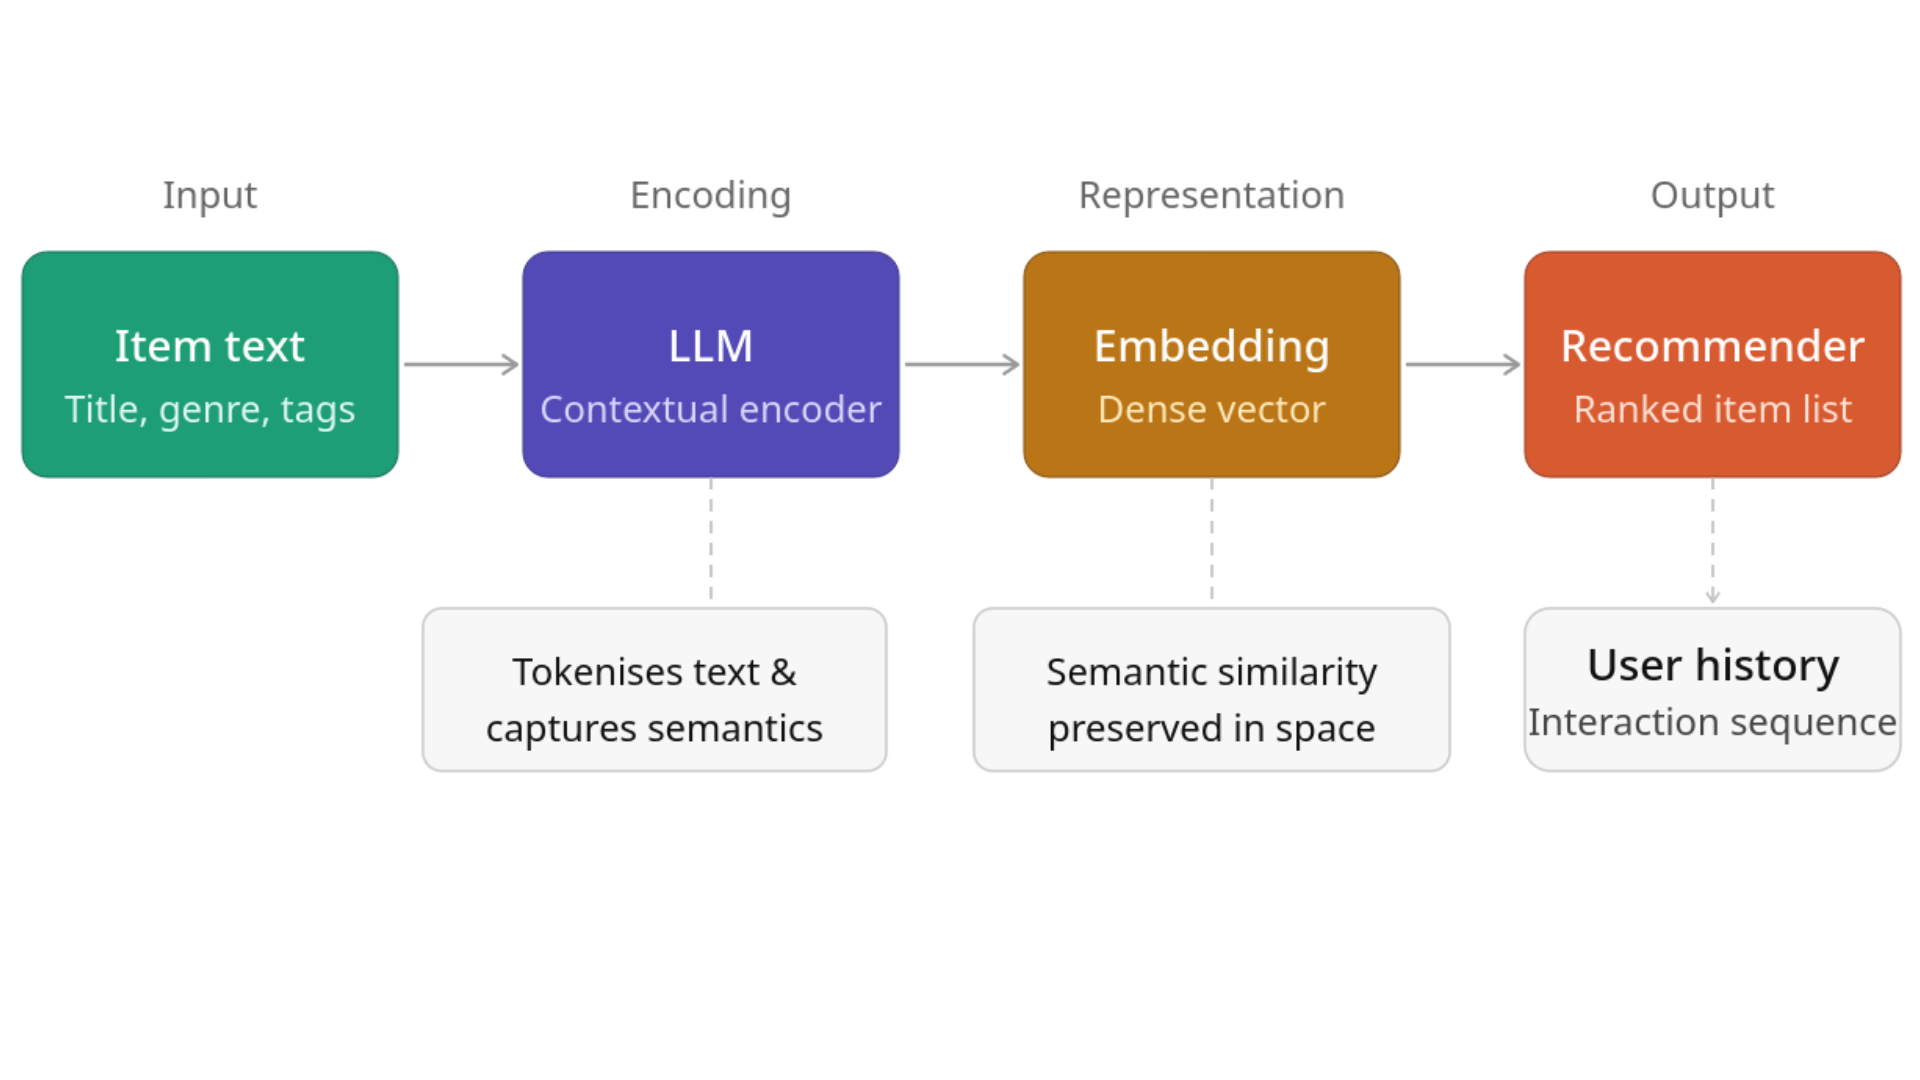
\includegraphics[width=0.92\textwidth]{picture/figures/schemas/llm_pipeline.png}
    % CORRECTION: shortened caption to one explicit line
    \caption{LLM pipeline for generating item embeddings used in a recommender.}
    \label{fig:llm_pipeline}
\end{figure}

\justifying
Recent studies have shown that LLMs can be used in several ways for sequential
recommendation. Some approaches initialize strong sequential models such as
BERT4Rec or SASRec with LLM-derived embeddings, while others fine-tune the LLM
directly for recommendation or use it as a semantic encoder for items and user
profiles \citep{harte2023leveraging,llmrec2024,wu2023survey}. Survey work also
highlights a broader shift from treating LLMs only as feature extractors toward
using them as integrated components of recommendation pipelines, including
knowledge enhancement, interaction enhancement, and model enhancement
\citep{liu2024llmers}. This makes LLMs a promising direction for improving both
representation quality and generalization in sequential recommendation.

At the same time, the usefulness of LLMs depends strongly on how item text is
constructed and presented. A short product title, a structured attribute list,
and a longer user-centric description can lead to different embedding spaces and
therefore different recommendation behaviors. For this reason, item text
design is not a trivial preprocessing step, but an important modeling choice
that can influence semantic richness, distinctiveness, and downstream
performance. This observation motivates the empirical study carried out in this
memoir, where different item description strategies are analyzed in the context
of sequential recommendation.

\begin{table}[h]
\centering
\begin{tabular}{p{3cm} p{3.5cm} p{6.3cm}}
\toprule
\textbf{Use case} & \textbf{Method} & \textbf{Key idea} \\
\midrule
Embedding initialization & LLM \(\rightarrow\) item vectors & Use semantic embeddings to initialize or enrich sequential recommenders. \\
Direct recommendation & LLM as recommender & Fine-tune or prompt the LLM to rank candidate items directly. \\
Hybrid enhancement & LLM + sequential model & Combine textual embeddings with behavioral sequence modeling. \\
\bottomrule
\end{tabular}
% CORRECTION: shortened table caption to one explicit line
\caption{Use cases of LLMs in sequential recommendation.}
\label{tab:llm_seq}
\end{table}


\section{Evaluation Metrics}

\justifying
To evaluate the performance of sequential recommendation models, this memoir
uses three standard ranking-based metrics: Hit Ratio at \(K\) (HR@K),
Normalized Discounted Cumulative Gain at \(K\) (NDCG@K), and Mean Reciprocal
Rank (MRR). These metrics measure how well the model places the true next item
among its top-ranked predictions. Since sequential recommendation is typically a
top-\(K\) ranking problem, such metrics are more informative than simple
classification accuracy.

\subsection{Hit Ratio at \(K\)}

HR@K measures whether the ground-truth next item appears in the top-\(K\)
recommended items. It gives a binary reward of 1 if the target item is present
in the recommendation list and 0 otherwise. As a result, HR@K captures the
model's ability to retrieve the correct item within a limited number of
suggestions, but it does not consider the exact rank position inside the top-\(K\).

\subsection{Normalized Discounted Cumulative Gain at \(K\)}

NDCG@K evaluates both whether the correct item is retrieved and how high it is
ranked in the recommendation list. Higher-ranked correct predictions receive
larger scores, which makes NDCG@K more sensitive to the ordering quality of the
top-\(K\) list. This metric is especially useful when the position of the
predicted item matters, which is often the case in practical recommendation
scenarios.

\subsection{Mean Reciprocal Rank}

MRR measures the inverse of the rank position of the first relevant item.
Unlike HR@K, it rewards models that place the target item very close to the top
of the list. If the correct item is ranked first, the reciprocal rank is 1; if
it is ranked second, it is \(1/2\), and so on. MRR therefore reflects how early
the desired item appears in the ranked output.

\begin{table}[h]
\centering
\begin{tabular}{p{2.5cm} p{5.2cm} p{5.5cm}}
\toprule
\textbf{Metric} & \textbf{Formula} & \textbf{What it measures} \\
\midrule
HR@K &
\[
\mathrm{HR@K} = \frac{1}{N}\sum_{i=1}^{N}\mathbb{I}(\text{rank}_i \leq K)
\]
&
Whether the true next item appears in the top-\(K\) recommendations. \\
\midrule
NDCG@K &
\[
\mathrm{NDCG@K} = \frac{1}{N}\sum_{i=1}^{N}\frac{\mathbb{I}(\text{rank}_i \leq K)}{\log_2(\text{rank}_i + 1)}
\]
&
Retrieval quality with a stronger reward for higher-ranked correct items. \\
\midrule
MRR &
\[
\mathrm{MRR} = \frac{1}{N}\sum_{i=1}^{N}\frac{1}{\text{rank}_i}
\]
&
How early the first relevant item appears in the ranked list. \\
\bottomrule
\end{tabular}
% CORRECTION: shortened table caption to one explicit line
\caption{Ranking metrics used for sequential recommendation evaluation.}
\label{tab:evaluation_metrics}
\end{table}

% ============================================================
% CORRECTION: Moved "Identified Gaps" BEFORE "Conclusion"
%             so that Conclusion appears last in the chapter.
% ============================================================

\section{Identified Gaps and Positioning of Contributions}

\justifying
Despite the substantial progress achieved by recent sequential recommendation
methods, two important gaps remain insufficiently addressed in the literature.
First, many hybrid GNN-Transformer approaches combine global graph signals and
local sequential signals using a fixed or uniform fusion strategy, without
considering that users exhibit different interaction history profiles. In
practice, users with sparse histories benefit more from global collaborative
information, whereas users with rich histories can better exploit detailed
sequential patterns. This observation motivates our first contribution, which
introduces a length-adaptive fusion mechanism that dynamically balances graph-
based and sequence-based representations according to the amount of available
user history.

Second, although large language models have recently been integrated into
recommendation systems, the influence of item textual description strategy on
the quality of the resulting embeddings has not yet been systematically
explored. Different forms of item text, such as titles, structured attributes,
or user-oriented descriptions, may produce embeddings with different semantic
properties and downstream effects on recommendation performance. This gap
motivates our second contribution, which conducts a systematic study of how item
description design affects LLM embeddings in sequential recommendation.

Together, these two gaps define the positioning of this memoir: the first
contribution addresses the adaptive fusion of structural and sequential signals,
while the second investigates the semantic role of item text in LLM-based
sequential recommendation.

\section{Conclusion}

\justifying
This chapter introduced the fundamental concepts underlying recommendation
systems and provided an overview of the main paradigms used in practice,
including collaborative filtering, sequence-based models, graph-based models,
and LLM-enhanced approaches. It also presented the sequential recommendation
setting, the principal baseline architectures used in this work, and the
evaluation metrics employed to assess model performance.

Despite the progress made by these methods, several limitations remain,
particularly in the way they model heterogeneous user histories, combine
global and local signals, and exploit textual item information. These open
questions motivate the research gaps addressed in the following chapter.


% ============================================================
%  CHAPTER 2 - Length-Adaptive Hybrid GNN-Transformer
% ============================================================
\chapter{Length-Adaptive Hybrid GNN-Transformer for Sequential Recommendation}

\section{Introduction}

\justifying
Sequential recommendation remains a challenging problem because user interaction
histories are heterogeneous in both length and density. Transformer-based models
such as SASRec \citep{kang2018sasrec} and BERT4Rec \citep{sun2019bert4rec} have
demonstrated strong performance by capturing long-range dependencies within
interaction sequences, but they rely on the availability of sufficiently long
histories to generalize reliably. Graph Neural Network models such as LightGCN
\citep{he2020lightgcn} address this by aggregating global collaborative signals
from the full user-item interaction graph, making them more robust for sparse
users. However, when used in isolation, each paradigm captures only one side of
the recommendation signal: sequence models ignore global item co-occurrence
structure, while graph models ignore the fine-grained temporal order of
individual user interactions \citep{wu2020gnnsurvey, pan2024survey}.

This chapter proposes a Length-Adaptive Hybrid GNN-Transformer, a model that
combines both paradigms through a user-specific fusion mechanism controlled by
the length of each user's interaction history. The core idea is that the
relative reliability of the graph signal versus the sequence signal is not
constant across users: it varies directly with the amount of available
sequential evidence. The proposed model quantifies this variation through a
scalar weight \(\lambda(u)\) that dynamically adjusts the contribution of the
GNN and Transformer branches for each user individually. The remainder of this
chapter is organized as follows: Section~\ref{sec:limitations} discusses the
limitations of existing models and formally states the research problem;
Section~\ref{sec:solution} introduces the adaptive fusion mechanism and the
formal problem definition; Section~\ref{sec:family} presents the family of
hybrid model variants; and Section~\ref{sec:ch2conclusion} concludes the
chapter.


\section{Limitations of Existing Models and Problem Statement}
\label{sec:limitations}

\justifying
Despite the progress achieved by the models reviewed in Chapter~1, three
concrete limitations can be identified in the existing literature on hybrid
GNN-Transformer sequential recommendation.

\textbf{Limitation 1 - Fixed fusion weights in existing hybrid models.}
Hybrid approaches that combine GNN and Transformer components, such as those
surveyed in \citep{wu2020gnnsurvey}, typically apply a single global fusion
weight that is shared uniformly across all users. This fixed weighting strategy
treats every user identically, regardless of how much interaction history is
available. As a result, the model cannot adapt to the fact that the relative
informativeness of the graph signal versus the sequence signal varies
substantially from one user to another. A fixed weight that is optimal on
average will systematically underserve both sparse users and dense users
\citep{pan2024survey}.

\textbf{Limitation 2 - Transformer-only models fail sparse users.}
Self-attention mechanisms, as used in SASRec \citep{kang2018sasrec} and
BERT4Rec \citep{sun2019bert4rec}, require a sufficient number of interactions
to produce reliable contextualized representations. When a user has only a
small number of past interactions, the self-attention layers lack enough context
to generalize, and the resulting sequence embedding is noisy or
underspecified. These models therefore provide poor recommendations for sparse
and cold-start users, a critical segment in any real-world recommendation
platform.

\textbf{Limitation 3 - GNN-only models waste dense users' sequential patterns.}
Graph-based models such as LightGCN \citep{he2020lightgcn} aggregate
neighborhood information over the full interaction graph and produce strong
collaborative embeddings for sparse users. However, they do not model the
temporal order of a user's individual interactions. For users with long, rich
interaction histories, this means that fine-grained sequential patterns --
the exact order in which items were consumed, recency effects, and evolving
preferences -- are entirely discarded. The graph signal alone is insufficient
to capture dynamic intent for active users \citep{pan2024survey}.

\subsection*{Problem Statement}

\justifying
The three limitations above converge on a single fundamental question, which
constitutes the first research problematic of this thesis:

\textit{How to dynamically adapt the fusion between global graph signals and
local sequential modelling according to each user's interaction history
profile?}

Answering this question requires a model that is aware of each user's
interaction density and uses this information to balance the GNN and
Transformer contributions at the individual user level, rather than applying
a fixed global weight. This is the design principle that motivates the
proposed architecture described in the following section.


% ============================================================
% CORRECTION: Section 2.3 "Proposed Solution" now opens with
%             an introductory paragraph + Figure 2.1 (architecture)
%             BEFORE the Formal Problem Definition subsection.
%             Figure moved here from Problem Statement section.
% ============================================================
\section{Proposed Solution: The Adaptive Fusion Mechanism}
\label{sec:solution}

\justifying
To overcome the limitations of fixed-weight fusion, we propose a length-adaptive
hybrid architecture that dynamically balances global graph signals and local
sequential patterns based on each user's interaction history length. The model
combines two complementary encoders: a Graph Neural Network (GNN) branch that
aggregates global collaborative signals from the full user-item interaction
graph, and a Transformer branch that models fine-grained sequential patterns
within each user's personal interaction history. The two branches are merged
through a user-specific fusion weight \(\lambda(u)\) that is automatically
derived from the length of the user's interaction history, ensuring that the
model adapts its balance between global and local information to each individual
user. Figure~\ref{fig:architecture} illustrates the overall architecture.

% CORRECTION: Figure moved from sec:limitations to here (Proposed Solution)
%             and caption updated to reflect it is the proposed architecture.
\begin{figure}[htbp]
    \centering
    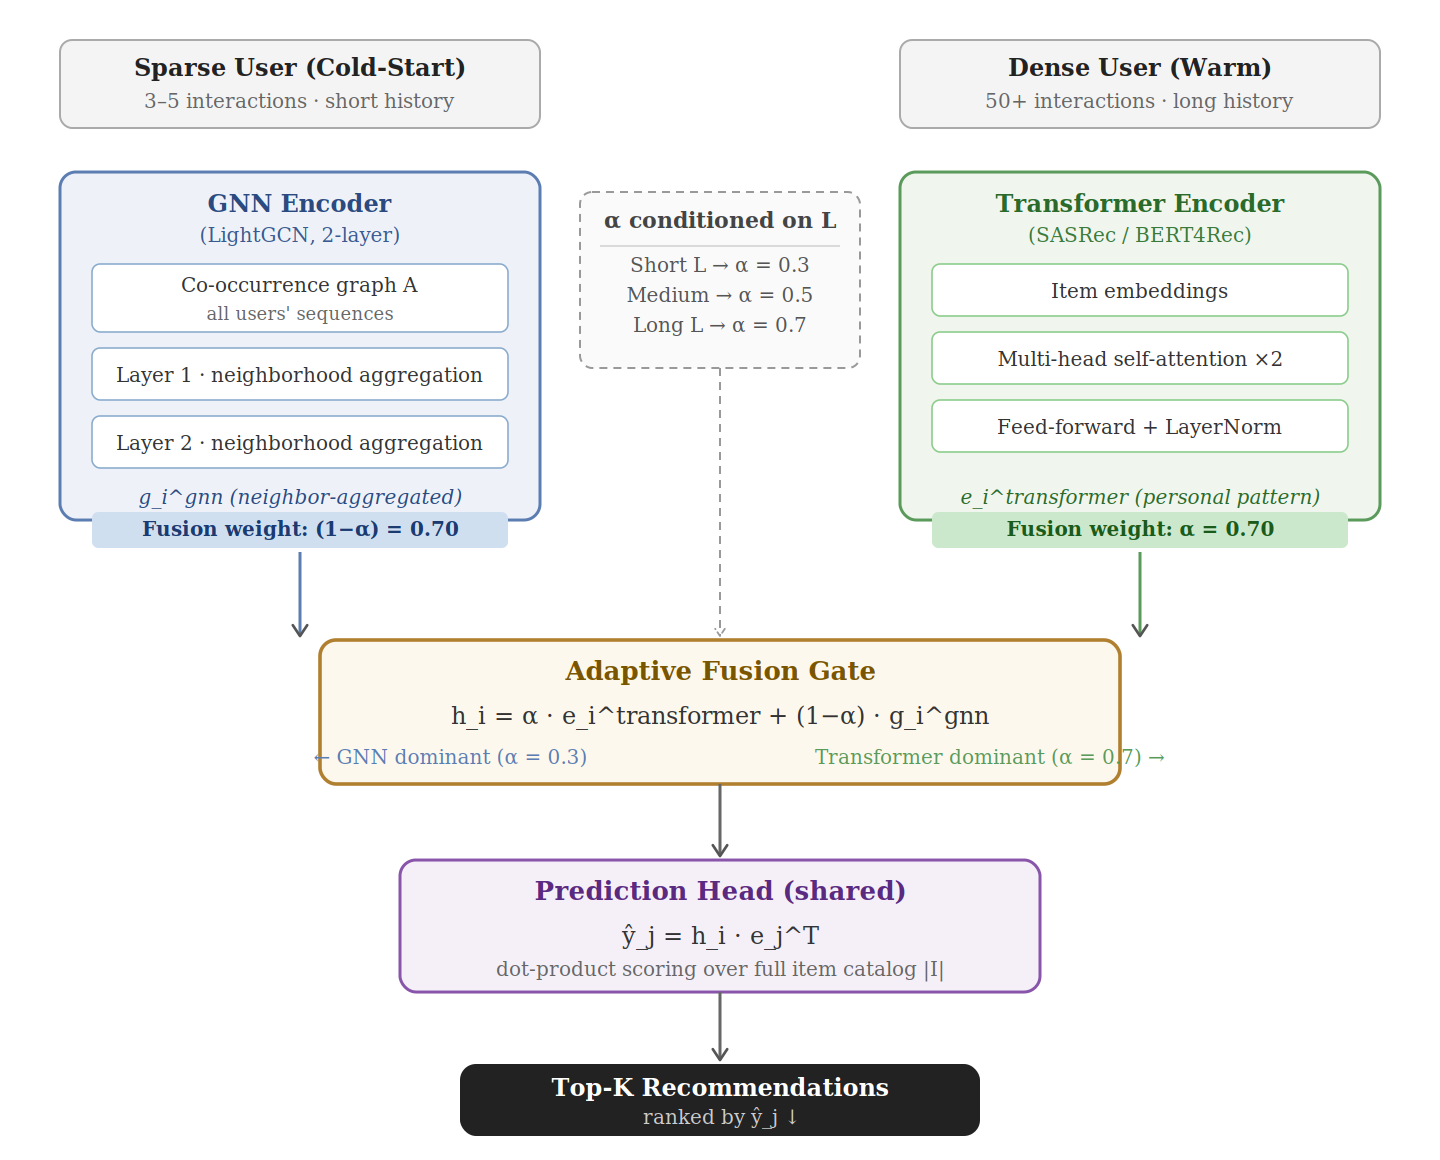
\includegraphics[width=1.15\textwidth]{picture/figures/schemas/sparse_dense_comparison.png}
    \caption{Proposed Architecture of the Length-Adaptive Hybrid GNN-Transformer.}
    \label{fig:architecture}
\end{figure}

\subsection{Formal Problem Definition}

\justifying
Let \(\mathcal{U}\) and \(\mathcal{I}\) denote the sets of users and items,
respectively. For each user \(u \in \mathcal{U}\), let
\(S_u = (i_1, i_2, \ldots, i_{n_u})\) be their interaction history of length
\(n_u\), where each \(i_t \in \mathcal{I}\) is an item consumed at time step
\(t\), ordered chronologically. The task of next-item sequential recommendation
is defined as: given the prefix \(S_u^{(t)} = (i_1, \ldots, i_t)\), learn a
scoring function

\begin{equation}
    f_{\Theta}\!\left(u,\, S_u^{(t)},\, j\right) \in \mathbb{R}
    \label{eq:scoring}
\end{equation}

\noindent that assigns a relevance score to each candidate item
\(j \in \mathcal{I}\), where \(\Theta\) denotes all trainable parameters. At
inference time, items are ranked by their scores and top-\(K\) accuracy is
evaluated via HR@\(K\), NDCG@\(K\), and MRR@\(K\) as defined in
Chapter~1.

\subsection{The Adaptive Fusion Mechanism}

\justifying
The proposed model computes two independent representations for each user
\(u\): a graph-based representation \(\mathbf{h}_u^{\text{GNN}}\), produced by
a Graph Neural Network encoder operating over the global item co-occurrence
graph, and a sequence-based representation \(\mathbf{h}_u^{\text{Trans}}\),
produced by a Transformer encoder operating over the user's personal
interaction history \(S_u\). These two representations are then combined
through a user-specific scalar weight \(\lambda(u) \in [0, 1]\):

\begin{equation}
    \mathbf{h}_u = \lambda(u)\cdot \mathbf{h}_u^{\text{Trans}}
    + \bigl(1 - \lambda(u)\bigr)\cdot \mathbf{h}_u^{\text{GNN}}
    \label{eq:fusion}
\end{equation}

\noindent where the fusion weight \(\lambda(u)\) is derived from the user's
interaction history length \(n_u\) and a normalization factor \(n_{\max}\),
the maximum history length observed in the training set:

\begin{equation}
    \lambda(u) = \sigma\!\left(\frac{n_u}{n_{\max}}\right)
    \label{eq:lambda}
\end{equation}

\noindent and \(\sigma(\cdot)\) denotes the sigmoid function
\(\sigma(x) = 1/(1 + e^{-x})\).

\subsection{Intuition and Rationale}

\justifying
The intuition behind Equations~\ref{eq:fusion} and~\ref{eq:lambda} is
straightforward. When a user has a short interaction history (\(n_u\) is
small), \(\lambda(u)\) is close to 0, and the fused representation
\(\mathbf{h}_u\) relies predominantly on \(\mathbf{h}_u^{\text{GNN}}\). This
is desirable because the GNN aggregates global co-occurrence signals from all
users in the training set and is therefore informative even when individual
sequence evidence is scarce. Conversely, when a user has a long interaction
history (\(n_u\) is large), \(\lambda(u)\) approaches 1, and \(\mathbf{h}_u\)
relies predominantly on \(\mathbf{h}_u^{\text{Trans}}\). In this regime, the
Transformer can exploit the full richness of the user's personal sequential
patterns, which carry more information than global averages.

The use of history length \(n_u\) as the proxy variable is motivated by the
observation that the reliability of self-attention degrades when the input
sequence is too short \citep{kang2018sasrec, sun2019bert4rec}, while GNN
neighborhood aggregation is length-independent by construction
\citep{he2020lightgcn}. The sigmoid normalization in
Equation~\ref{eq:lambda} ensures that \(\lambda(u)\) remains bounded in
\([0, 1]\) and transitions smoothly between the two extremes, avoiding hard
discontinuities in the embedding space.


\section{Family of Proposed Hybrid Models}
\label{sec:family}
\justifying

This work proposes four hybrid models, all built on the same core idea:
combining a graph encoder with a sequential encoder, and blending their
outputs based on how long a user's interaction history is. The models share
the same LightGCN~\citep{he2020lightgcn} graph backbone and differ in how
they encode sequences and how they control the blending.

% CORRECTION: clarified difference between Fixed and Discrete fusion strategies
\subsection{Hybrid BERT4Rec + LightGCN with Fixed Fusion}
\label{sec:fixed}

\justifying
The simplest variant applies a single fixed blending weight \(\alpha\) to all
users equally, regardless of their individual history lengths. LightGCN provides
collaborative signals from the item co-occurrence graph, while
BERT4Rec~\citep{sun2019bert4rec} encodes the interaction sequence using
bidirectional self-attention. The value of \(\alpha\) is set manually before
training and remains constant throughout: every user receives the same relative
contribution from the GNN and Transformer branches. This model serves as the
baseline of the family, confirming that combining the two encoders is beneficial,
but it cannot adapt to the heterogeneity of user histories.

\subsection{Hybrid BERT4Rec + LightGCN with Discrete Fusion}
\label{sec:discrete}

\justifying
\textbf{Fixed Fusion} applies a single, global scalar weight \(\alpha\) to all
users. This weight is set manually before training and does not vary across
users, regardless of their history length. In contrast, \textbf{Discrete Fusion}
first divides users into three groups based on their history length (short,
medium, long). Each group receives its own manually tuned weight
(\(\alpha_{\text{short}}, \alpha_{\text{mid}}, \alpha_{\text{long}}\)), which is
fixed during training. Thus, Discrete Fusion is history-aware but not adaptive
at the individual user level, whereas Fixed Fusion is fully uniform across all
users and ignores history length entirely. The discrete variant is therefore more
principled than the fixed variant because it acknowledges that different user
profiles need different balances, while adding no trainable parameters and
remaining fully interpretable.

\subsection{Hybrid BERT4Rec + Temporal Graph Transformer (TGT)}
\label{sec:tgt}

% CORRECTION: added reference for TGT (Temporal Graph Transformer)
\justifying
This variant replaces LightGCN with a Temporal Graph Transformer inspired by
TGAT~\cite{xu2020tgat}, adapted here as a sequence encoder with a dual
attention pathway and a learnable cosine time encoding
$\cos(\mathbf{W} \cdot t)$. Recent works such as Temporal Graph Networks
(TGN)~\cite{rossi2020tgn} and Temporal Convolutional Transformer
(TCT)~\cite{tct2021placeholder} have also addressed temporal dynamics in
graphs. Concretely, it augments the attention keys with learned time encodings
so that the model can weigh recent interactions more heavily than older ones
when building item representations. BERT4Rec handles the sequential side as
before. The two branches are fused through a single learnable gating parameter
that is optimised during training, allowing the model to find the right balance
automatically. This makes TGT-BERT4Rec the most expressive graph-based hybrid
in the family, at the cost of higher complexity.

\subsection{Hybrid BERT4Rec + Temporal Convolutional Network (TCN)}
\label{sec:tcn}

% CORRECTION: added reference for TCN (Temporal Convolutional Network)
\justifying
The TCN variant replaces the graph encoder entirely with a Temporal
Convolutional Network \citep{bai2018tcn}. TCN uses stacked dilated causal
convolutions, meaning it can capture long-range sequential dependencies without
ever looking at future tokens. Because convolutions process sequences much faster
than attention, this model is significantly more efficient than the
transformer-only alternatives. The TCN and BERT4Rec branches share the same
item embeddings and their outputs are combined through either a fixed weight, a
learnable scalar, or a learned projection layer that concatenates both
representations. This variant is particularly useful when inference speed or
memory is a constraint.

\begin{table}[h]
\centering
% CORRECTION: shortened table caption to one explicit line
\caption{Overview of the four proposed hybrid model variants.}
\label{tab:model_family}
\begin{tabular}{p{3.8cm} p{3.2cm} p{2.8cm} p{3.0cm}}
\toprule
\textbf{Model} & \textbf{Graph / Conv encoder} & \textbf{Seq.\ encoder} & \textbf{Fusion} \\
\midrule
Fixed Fusion       & LightGCN   & BERT4Rec & Fixed scalar, same for all users \\[3pt]
Discrete Fusion    & LightGCN   & BERT4Rec & Fixed scalar per length group \\[3pt]
TGT-BERT4Rec       & Temporal Graph Transformer & BERT4Rec & Learned gate \\[3pt]
TCN-BERT4Rec       & Temporal Conv.\ Network & BERT4Rec & Fixed / learned / concat \\
\bottomrule
\end{tabular}
\end{table}

\section{Conclusion}
\label{sec:ch2conclusion}

\justifying
This chapter proposed a Length-Adaptive Hybrid GNN-Transformer framework for
sequential recommendation, built around the core idea that the optimal balance
between global graph signals and local sequential signals is not constant but
varies with each user's interaction history length. The novelty of the proposed
approach lies in the user-specific fusion weight \(\lambda(u)\), which
dynamically shifts the representation from GNN-dominated for sparse users
toward Transformer-dominated for dense users, addressing a design flaw shared
by all existing fixed-weight hybrid models \citep{wu2020gnnsurvey,
pan2024survey}. Two concrete variants were derived from this framework by
combining LightGCN \citep{he2020lightgcn} with BERT4Rec
\citep{sun2019bert4rec}, and using either a linear or sigmoid fusion schedule,
allowing the effect of the fusion schedule choice to be studied independently.
A current limitation of the framework is that \(\lambda(u)\) is computed from
history length alone using a fixed formula, rather than being learned
end-to-end from data, which may leave performance gains on the table for users
whose optimal fusion point does not align perfectly with their history length.
The experimental validation of both variants, including comparisons against the
baseline models from Chapter~1 and a per-user-segment analysis, is presented
in Chapter~3.

% ============================================================
%  CHAPTER 3 - Experiments and Results (Contribution 1)
% ============================================================
\chapter{Experiments and Results: Length-Adaptive Hybrid GNN-Transformer}

% CORRECTION: removed the publication note paragraph as requested

\section{Introduction}

\justifying
Chapter~2 proposed a Length-Adaptive Hybrid GNN-Transformer framework for
sequential recommendation, built around the idea that the relative contribution
of global graph signals and local sequential signals should vary according to
each user's interaction history length. The framework was instantiated into two
concrete model variants combining LightGCN \citep{he2020lightgcn} with
BERT4Rec \citep{sun2019bert4rec}, using either a linear or sigmoid fusion
schedule for \(\lambda(u)\). This chapter provides the empirical validation of
these two variants against a set of strong sequential and graph-based baselines
on two standard benchmark datasets.

The experiments in this chapter are designed to answer three concrete
questions. First, does the proposed adaptive fusion mechanism yield better
overall recommendation performance compared to fixed-weight hybrid baselines
and to single-paradigm models? Second, does the length-adaptive design
specifically improve performance for sparse users, who are systematically
underserved by Transformer-only models? Third, does each component of the
proposed architecture -- the GNN branch, the Transformer branch, and the
adaptive \(\lambda(u)\) schedule -- contribute independently to the final
performance, or can any of them be removed without degrading results?

The remainder of this chapter is organized as follows.
Section~\ref{sec:datasets} describes the datasets used and justifies their
selection. Section~\ref{sec:preprocessing} details the preprocessing pipeline.
Section~\ref{sec:hyperparameters} reports all hyperparameter settings.
Section~\ref{sec:baselines} presents the baseline models and the evaluation
protocol. Section~\ref{sec:results} reports and analyzes the main results.
Section~\ref{sec:ablation} presents the ablation study. Finally,
Section~\ref{sec:ch3conclusion} concludes the chapter and transitions to
Chapter~4.

\section{Datasets}
\label{sec:datasets}

\justifying
The experiments are conducted on two standard sequential recommendation
benchmarks derived from the MovieLens collection \citep{harper2015movielens},
which are among the most widely used datasets in the sequential recommendation
literature \citep{pan2024survey, kang2018sasrec, sun2019bert4rec}. These
datasets were chosen because they cover two different scales of interaction
density, allowing the evaluation of model robustness across both sparse and
dense user populations -- a property that is particularly important for
validating the length-adaptive design of the proposed model.

\textbf{MovieLens-100K (ML-100K)} contains 100,000 explicit ratings collected
from 943 users on 1,682 movies. After filtering users with fewer than 5
interactions and converting ratings to implicit feedback (an interaction is
recorded if and only if the rating is \(\geq 4\)), the dataset yields 938 test users. This
smaller dataset contains a higher proportion of sparse users relative to
ML-1M, making it a valuable testbed for evaluating cold-start and sparse-user
behavior.

\textbf{MovieLens-1M (ML-1M)} contains approximately 1 million ratings from
6,040 users on 3,706 movies. After the same preprocessing steps, the dataset
yields 6,034 test users. Its larger scale and denser interaction distribution
make it a complementary benchmark to ML-100K, allowing the evaluation of
model scalability and performance under richer sequential evidence.

\begin{table}[h]
\centering
% CORRECTION: shortened table caption to one explicit line
\caption{Dataset statistics after preprocessing.}
\label{tab:datasets}
\begin{tabular}{p{2.8cm} p{1.8cm} p{1.8cm} p{2.5cm} p{2.2cm} p{2.2cm}}
\toprule
\textbf{Dataset} & \textbf{\#Users} & \textbf{\#Items} &
\textbf{\#Interactions} & \textbf{Sparsity} & \textbf{Avg. seq. length} \\
\midrule
ML-100K & 943  & 1,682 & 100,000   & 93.70\% & 106.0 \\
ML-1M   & 6,040 & 3,706 & 1,000,209 & 95.53\% & 165.5 \\
\bottomrule
\end{tabular}
\end{table}

\noindent Sparsity is computed as
\(1 - \frac{\text{\#Interactions}}{\text{\#Users} \times \text{\#Items}}\).
Both datasets confirm the typical sparsity challenge in collaborative filtering,
motivating the use of GNN signals to supplement sequential evidence for users
with short histories.

\section{Preprocessing}
\label{sec:preprocessing}

\justifying
The raw MovieLens datasets are preprocessed following the standard pipeline
used in the sequential recommendation literature
\citep{kang2018sasrec, sun2019bert4rec, pan2024survey}. The preprocessing
steps are applied identically to both ML-100K and ML-1M to ensure fair
comparison across datasets. The full pipeline is illustrated in
Figure~\ref{fig:preprocessing}.

\begin{figure}[H]
    \centering
    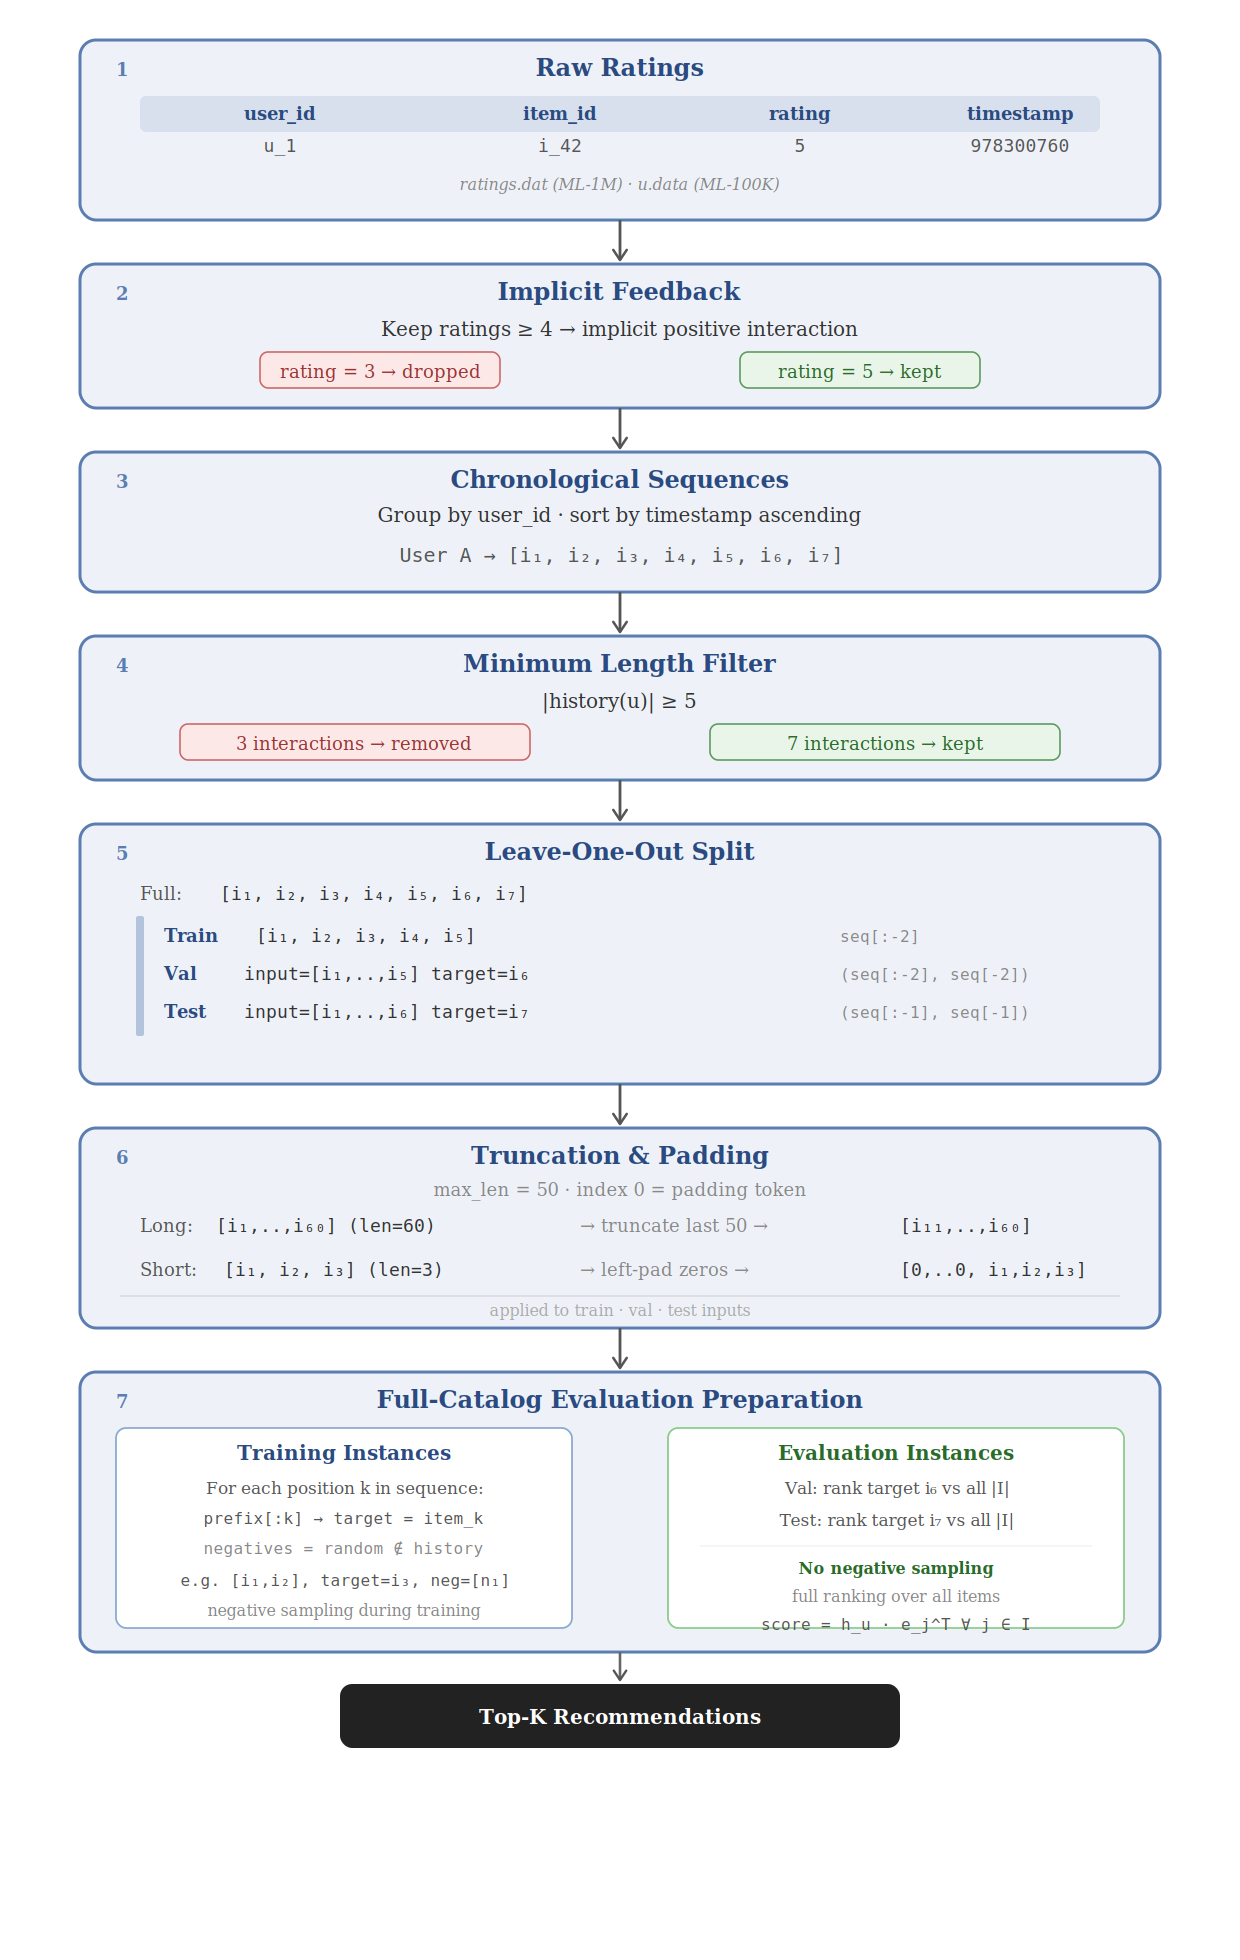
\includegraphics[width=0.9\textwidth]{picture/figures/schemas/preprocessing_pipeline.png}
    % CORRECTION: shortened caption to one explicit line
    \caption{Standard preprocessing pipeline applied to both datasets.}
    \label{fig:preprocessing}
\end{figure}

\textbf{Step 1 - Implicit feedback conversion.}
All explicit ratings are converted to implicit feedback: an interaction is
recorded if and only if the rating value is greater than or equal to 4. This
binary conversion is standard in sequential recommendation, where the goal is
to model the order of consumed items rather than preference intensity.

\textbf{Step 2 - 5-core filtering.}
Users and items with fewer than 5 interactions are removed from the dataset.
This filtering step ensures that every user has enough interaction history to
construct a meaningful training sequence, and that every item appears
sufficiently often to learn a reliable embedding. The filter is applied
iteratively until no user or item falls below the threshold.

\textbf{Step 3 - Chronological sorting.}
For each user, all interactions are sorted in ascending order of timestamp.
This produces a chronologically ordered interaction sequence
\(S_u = (i_1, i_2, \ldots, i_{n_u})\) for each user \(u\), which is the
input format required by all sequential models.

\textbf{Step 4 - Leave-one-out split.}
The dataset is split into training, validation, and test sets following the
leave-one-out protocol \citep{kang2018sasrec}. For each user, the last item
in the interaction sequence is held out for testing, the second-to-last item
is held out for validation, and all remaining items form the training set.
This protocol is standard in the sequential recommendation literature and
ensures that the temporal order of interactions is preserved.

\textbf{Step 5 - Sequence truncation.}
To manage computational cost, interaction sequences are truncated to a maximum
length of 200 for hybrid models and 50 for pure sequential baselines. When a
sequence exceeds the maximum length, the most recent interactions are retained
and earlier ones are discarded, preserving the most informative recent context.

\textbf{Step 6 - Negative sampling for evaluation.}
During evaluation, each positive test item is ranked against all items in the
full item catalog. No negative sampling is applied at test time, ensuring that
the reported metrics reflect full-catalog ranking performance rather than
sampled approximations. During training, 100 negative items are sampled
uniformly at random per positive interaction for the binary cross-entropy loss.


\section{Hyperparameters}
\label{sec:hyperparameters}

\justifying
All models are implemented and trained under identical conditions to ensure
fair comparison. The hyperparameters used in this chapter are reported in
Table~\ref{tab:hyperparameters}. General architecture hyperparameters --
embedding dimension, number of attention heads, number of Transformer blocks,
and dropout rate -- are fixed to the same values across all models. Training
hyperparameters -- optimizer, learning rate, batch size, and early stopping
criterion -- are also held constant. This design ensures that any observed
performance differences between models are attributable to architectural
choices rather than training configuration differences.

The GNN-specific hyperparameters -- number of GCN layers and co-occurrence
graph construction parameters -- are fixed based on standard settings from
the LightGCN literature \citep{he2020lightgcn}. The co-occurrence window size
\(w = 5\) and minimum co-occurrence threshold \(\tau = 2\) were chosen to
balance graph density and edge quality: a window that is too narrow misses
meaningful item relationships, while a threshold that is too low introduces
noisy edges that degrade embedding quality.

For the HybridDiscrete variant, the three fusion weight values
\(\alpha_{\text{short}}\), \(\alpha_{\text{mid}}\), and \(\alpha_{\text{long}}\)
are treated as hyperparameters tuned on the validation set using
NDCG@10 as the selection criterion. The history length thresholds
\(L^*_{\text{short}} = 10\) and \(L^*_{\text{long}} = 30\) partition users
into three bins and were selected based on the empirical distribution of
history lengths in the training set.

\begin{table}[h]
\centering
% CORRECTION: shortened table caption to one explicit line
\caption{Hyperparameter settings for all models.}
\label{tab:hyperparameters}
\begin{tabular}{p{5.5cm} p{2.5cm} p{4.5cm}}
\toprule
\textbf{Hyperparameter} & \textbf{Value} & \textbf{Search range / Note} \\
\midrule
\multicolumn{3}{l}{\textit{General}} \\
Embedding dimension \(d\)       & 64      & Fixed \\
Attention heads                 & 2       & Fixed \\
Transformer blocks \(B\)        & 2       & Fixed \\
Dropout rate                    & 0.2     & Fixed \\
Max sequence length (hybrid)    & 200     & Fixed \\
Max sequence length (baselines) & 50      & Fixed \\
\midrule
\multicolumn{3}{l}{\textit{Training}} \\
Optimizer                       & Adam    & Fixed \\
Learning rate \(\eta\)          & 0.001   & Fixed \\
Batch size                      & 256     & Fixed \\
Max epochs                      & 200     & Fixed \\
Early stopping patience         & 20      & Validation NDCG@10 \\
Negatives per positive          & 100     & Fixed \\
\midrule
\multicolumn{3}{l}{\textit{GNN Encoder}} \\
GCN layers \(L_{\text{GNN}}\)   & 2       & Fixed \\
Co-occurrence window \(w\)      & 5       & Fixed \\
Min co-occurrence threshold \(\tau\) & 2  & Fixed \\
\midrule
\multicolumn{3}{l}{\textit{HybridDiscrete Fusion}} \\
Short-history threshold \(L^*_{\text{short}}\) & 10 & Fixed \\
Long-history threshold \(L^*_{\text{long}}\)   & 30 & Fixed \\
\(\alpha_{\text{short}}\)       & 0.3     & Tuned on validation set \\
\(\alpha_{\text{mid}}\)         & 0.5     & Tuned on validation set \\
\(\alpha_{\text{long}}\)        & 0.7     & Tuned on validation set \\
\midrule
\multicolumn{3}{p{\linewidth}}{\footnotesize
*TCN-BERT4Rec and TGT-BERT4Rec use the same general hyperparameters
(embedding dim 64, 2 heads, 2 blocks, dropout 0.2).
} \\
\bottomrule
\end{tabular}
\end{table}

\section{Baselines}
\label{sec:baselines}

\justifying
The proposed hybrid model variants are evaluated against five baseline models
grouped into three categories: sequential-only models, a graph-only model, and
hybrid ablation variants derived from the proposed framework itself. All models
are evaluated using the leave-one-out protocol described in
Section~\ref{sec:preprocessing}, where each positive test item is ranked
against all items in the full catalog. Performance is reported at cut-off
\(K \in \{5, 10, 20\}\) for HR@\(K\), NDCG@\(K\), and MRR@\(K\).

\subsection*{Sequential-Only Baselines}

\textbf{GRU4Rec} \citep{hidasi2016gru4rec} is a recurrent neural network model
that uses gated recurrent units to process interaction sequences step by step,
capturing short-term session-level dynamics. It serves as the recurrent
baseline and represents the earliest class of deep sequential recommendation
models.

\textbf{SASRec} \citep{kang2018sasrec} applies unidirectional causal
self-attention to model long-range dependencies in interaction sequences. It is
trained with binary cross-entropy loss and is one of the strongest and most
widely adopted Transformer-based baselines in sequential recommendation.

\textbf{BERT4Rec} \citep{sun2019bert4rec} uses bidirectional self-attention and
a masked item prediction objective to produce rich contextual sequence
representations. It is the sequential backbone shared by all proposed hybrid
variants and serves as the primary baseline against which the hybrid framework
is evaluated.

\textbf{Caser} \citep{tang2018caser} applies horizontal and vertical
convolutional filters over a sequence-as-image representation to capture both
point-level and union-level sequential patterns. It represents the
convolutional family of sequential models.

\subsection*{Graph-Only Baseline}

\textbf{LightGCN} \citep{he2020lightgcn} simplifies graph convolution to pure
neighborhood aggregation over the user-item bipartite graph, without feature
transformation or nonlinear activation. It is included not as a competitive
sequential baseline but as a reference point that isolates the contribution of
pure collaborative filtering signals in a next-item prediction setting. Its
relatively low performance on sequential metrics directly motivates the hybrid
design: static graph-based collaborative filtering alone is insufficient when
temporal ordering matters.

\subsection*{Hybrid Ablation Variants}

The following three variants of the proposed framework are included as internal
ablation baselines to isolate the contribution of each architectural component:

\textbf{HybridFixed} uses a single global fusion weight \(\alpha\) shared
uniformly across all users, trained end-to-end as a learnable scalar. It
verifies that combining GNN and Transformer embeddings is beneficial, while
treating every user identically regardless of history length.

\textbf{TCN-BERT4Rec} replaces the GCN graph encoder with a dilated causal
convolutional network that encodes local sequential transition patterns. It
tests whether local convolutional features provide complementary information
to the global self-attention of BERT4Rec, without relying on a pre-built item
graph.

\textbf{TGT-BERT4Rec} augments the item co-occurrence graph with temporal
information by encoding interaction timestamps as continuous time embeddings,
and combines the temporal graph encoder output with BERT4Rec using a learnable
gated fusion. It is particularly suited to short-history users whose temporal
patterns encode strong preference signals even when interaction counts are low.

\begin{table}[h]
\centering
% CORRECTION: shortened table caption to one explicit line
\caption{Summary of baseline models used in this chapter.}
\label{tab:baselines}
\begin{tabular}{p{3.2cm} p{2.5cm} p{7.0cm}}
\toprule
\textbf{Model} & \textbf{Category} & \textbf{Key characteristic} \\
\midrule
GRU4Rec   & Sequential & Gated recurrent units for session-level dynamics \\
Caser     & Sequential & Convolutional filters over sequence-as-image \\
SASRec    & Sequential & Unidirectional causal self-attention \\
BERT4Rec  & Sequential & Bidirectional masked item prediction \\
LightGCN  & Graph      & Pure neighborhood aggregation on bipartite graph \\
HybridFixed    & Hybrid ablation & Fixed global fusion weight for all users \\
TCN-BERT4Rec   & Hybrid ablation & Temporal convolution + BERT4Rec \\
TGT-BERT4Rec   & Hybrid ablation & Temporal graph encoder + BERT4Rec \\
\bottomrule
\end{tabular}
\end{table}

\section{Main Results Tables}
\label{sec:results_tables}

Table~\ref{tab:results_ml1m} and Table~\ref{tab:results_ml100k} report the
main results on ML-1M and ML-100K respectively. Bold values indicate the best
result per column and underlined values indicate the second best. The proposed
hybrid variants are marked with \(\bullet\). Results are reported at cut-off
\(K \in \{5, 10, 20\}\) for HR@\(K\), NDCG@\(K\), and MRR@\(K\).

\begin{table}[h]
\centering
% CORRECTION: shortened table caption to one explicit line
\caption{Test performance on MovieLens-1M (best in bold, second-best underlined).}
\label{tab:results_ml1m}
\resizebox{\textwidth}{!}{%
\begin{tabular}{p{3.5cm} ccc ccc ccc}
\toprule
& \multicolumn{3}{c}{\textbf{HR@K}} &
  \multicolumn{3}{c}{\textbf{NDCG@K}} &
  \multicolumn{3}{c}{\textbf{MRR@K}} \\
\cmidrule(lr){2-4}\cmidrule(lr){5-7}\cmidrule(lr){8-10}
\textbf{Model} &
@5 & @10 & @20 & @5 & @10 & @20 & @5 & @10 & @20 \\
\midrule
GRU4Rec   & 0.0365 & 0.0708 & 0.1173 & 0.0214 & 0.0324 & 0.0440 & 0.0165 & 0.0210 & 0.0241 \\
LightGCN  & 0.0121 & 0.0247 & 0.0467 & 0.0065 & 0.0106 & 0.0161 & 0.0047 & 0.0064 & 0.0079 \\
Caser     & 0.0684 & 0.1260 & 0.2135 & 0.0397 & 0.0581 & 0.0801 & 0.0303 & 0.0379 & 0.0438 \\
SASRec    & 0.0515 & 0.0979 & 0.1767 & 0.0298 & 0.0446 & 0.0643 & 0.0228 & 0.0287 & 0.0340 \\
BERT4Rec  & 0.0757 & 0.1374 & 0.2274 & 0.0453 & 0.0652 & 0.0879 & 0.0354 & 0.0437 & 0.0498 \\
\midrule
TCN-BERT4Rec\(^\bullet\)   & 0.0754 & 0.1385 & 0.2325 & 0.0449 & 0.0652 & 0.0888 & 0.0350 & 0.0433 & 0.0498 \\
TGT-BERT4Rec\(^\bullet\)   & 0.0820 & \underline{0.1480} & \underline{0.2444} & 0.0477 & \underline{0.0689} & \underline{0.0930} & 0.0365 & \underline{0.0452} & \underline{0.0517} \\
HybridDiscrete\(^\bullet\) & 0.0832 & 0.1427 & 0.2317 & 0.0492 & 0.0682 & 0.0905 & 0.0381 & 0.0459 & 0.0519 \\
HybridFixed\(^\bullet\)    & \textbf{0.0852} & \textbf{0.1485} & \textbf{0.2511} & \textbf{0.0524} & \textbf{0.0727} & \textbf{0.0984} & \textbf{0.0417} & \textbf{0.0499} & \textbf{0.0569} \\
\bottomrule
\end{tabular}}
\end{table}

\begin{table}[h]
\centering
% CORRECTION: shortened table caption to one explicit line
\caption{Test performance on MovieLens-100K (best in bold, second-best underlined).}
\label{tab:results_ml100k}
\resizebox{\textwidth}{!}{%
\begin{tabular}{p{3.5cm} ccc ccc ccc}
\toprule
& \multicolumn{3}{c}{\textbf{HR@K}} &
  \multicolumn{3}{c}{\textbf{NDCG@K}} &
  \multicolumn{3}{c}{\textbf{MRR@K}} \\
\cmidrule(lr){2-4}\cmidrule(lr){5-7}\cmidrule(lr){8-10}
\textbf{Model} &
@5 & @10 & @20 & @5 & @10 & @20 & @5 & @10 & @20 \\
\midrule
GRU4Rec   & 0.0341 & 0.0650 & 0.1077 & 0.0201 & 0.0302 & 0.0411 & 0.0156 & 0.0198 & 0.0229 \\
LightGCN  & 0.0320 & 0.0682 & 0.1194 & 0.0196 & 0.0312 & 0.0441 & 0.0155 & 0.0202 & 0.0237 \\
Caser     & 0.0576 & 0.1109 & 0.1844 & 0.0369 & 0.0540 & 0.0726 & 0.0302 & 0.0371 & 0.0422 \\
SASRec    & 0.0416 & 0.0682 & 0.1461 & 0.0255 & 0.0339 & 0.0532 & 0.0202 & 0.0235 & 0.0286 \\
BERT4Rec  & 0.0565 & 0.0949 & 0.1844 & 0.0327 & 0.0449 & 0.0671 & 0.0250 & 0.0299 & 0.0358 \\
\midrule
TCN-BERT4Rec\(^\bullet\)   & 0.0682 & \textbf{0.1194} & \textbf{0.2111} & \textbf{0.0386} & \underline{0.0551} & \textbf{0.0780} & \textbf{0.0290} & \underline{0.0358} & \textbf{0.0419} \\
TGT-BERT4Rec\(^\bullet\)   & 0.0512 & 0.0981 & 0.1684 & 0.0340 & 0.0490 & 0.0665 & 0.0284 & 0.0345 & 0.0391 \\
HybridDiscrete\(^\bullet\) & 0.0512 & 0.0853 & 0.1535 & 0.0291 & 0.0402 & 0.0575 & 0.0219 & 0.0266 & 0.0313 \\
HybridFixed\(^\bullet\)    & \textbf{0.0501} & \underline{0.0864} & \underline{0.1727} & \underline{0.0279} & 0.0393 & \underline{0.0610} & \underline{0.0207} & 0.0252 & \underline{0.0311} \\
\bottomrule
\end{tabular}}
\end{table}

\section{Experimental Results}
\label{sec:results}

\justifying
This section presents the evaluation results on both datasets across
all metrics and model variants. Results are organized around two
complementary views: a full metric heatmap and a per-history-length
breakdown.

% CORRECTION: removed Generalization Analysis subsection and its figures

\subsection{Overall Test Metrics}

\begin{figure}[H]
    \centering
    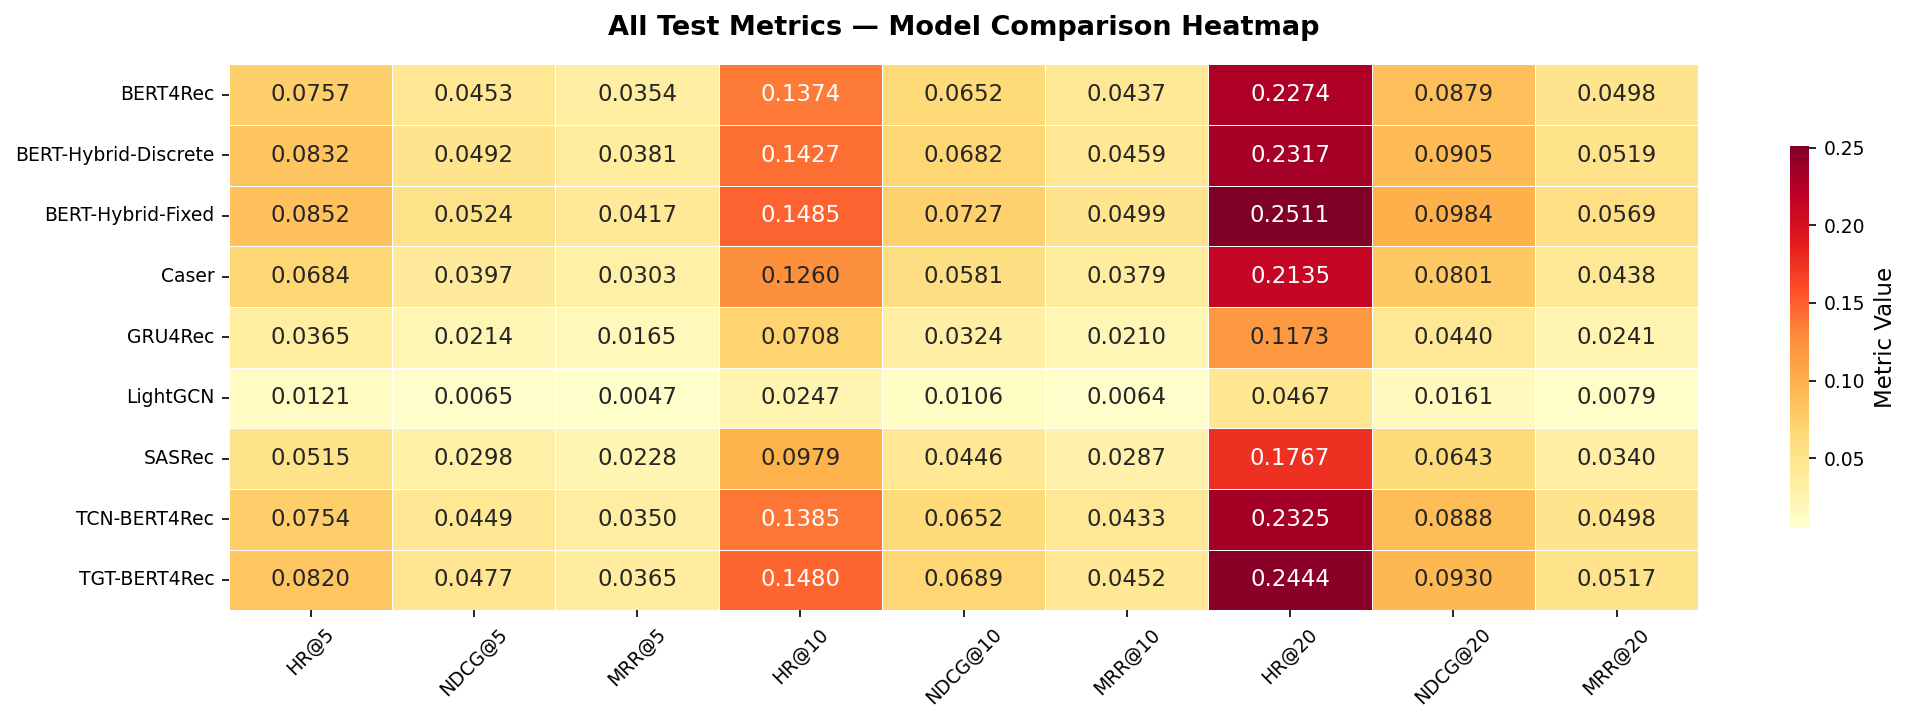
\includegraphics[width=0.95\textwidth]{picture/figures/1m/heatmap_all_test_metrics_1m.png}
    % CORRECTION: shortened caption to one explicit line
    \caption{Test metrics heatmap on ML-1M (darker cells indicate higher values).}
    \label{fig:heatmap_1m}
\end{figure}

\justifying
On ML-1M (Figure~\ref{fig:heatmap_1m}), the hybrid variants occupy the
top three rows of the heatmap across nearly every metric and cut-off.
\textbf{BERT-Hybrid-Fixed} achieves the strongest overall performance
with HR@10~\(= 0.1485\), NDCG@10~\(= 0.0727\), and MRR@10~\(= 0.0499\),
representing gains of \(+8.1\%\), \(+11.5\%\), and \(+14.2\%\) respectively
over the BERT4Rec baseline. \textbf{TGT-BERT4Rec} ranks second in most
columns and records the highest HR@20~\(= 0.2444\) across all models,
suggesting that temporal graph signals become especially valuable when
the recommendation list is extended. \textbf{BERT-Hybrid-Discrete}
improves over BERT4Rec on every metric despite using a simple
fixed-threshold fusion, directly validating the length-adaptive design
principle. \textbf{LightGCN} records the weakest performance overall
(HR@10~\(= 0.0247\)), confirming that pure graph-based collaborative
filtering is insufficient in a sequential setting where temporal order
carries important information.

\begin{figure}[H]
    \centering
    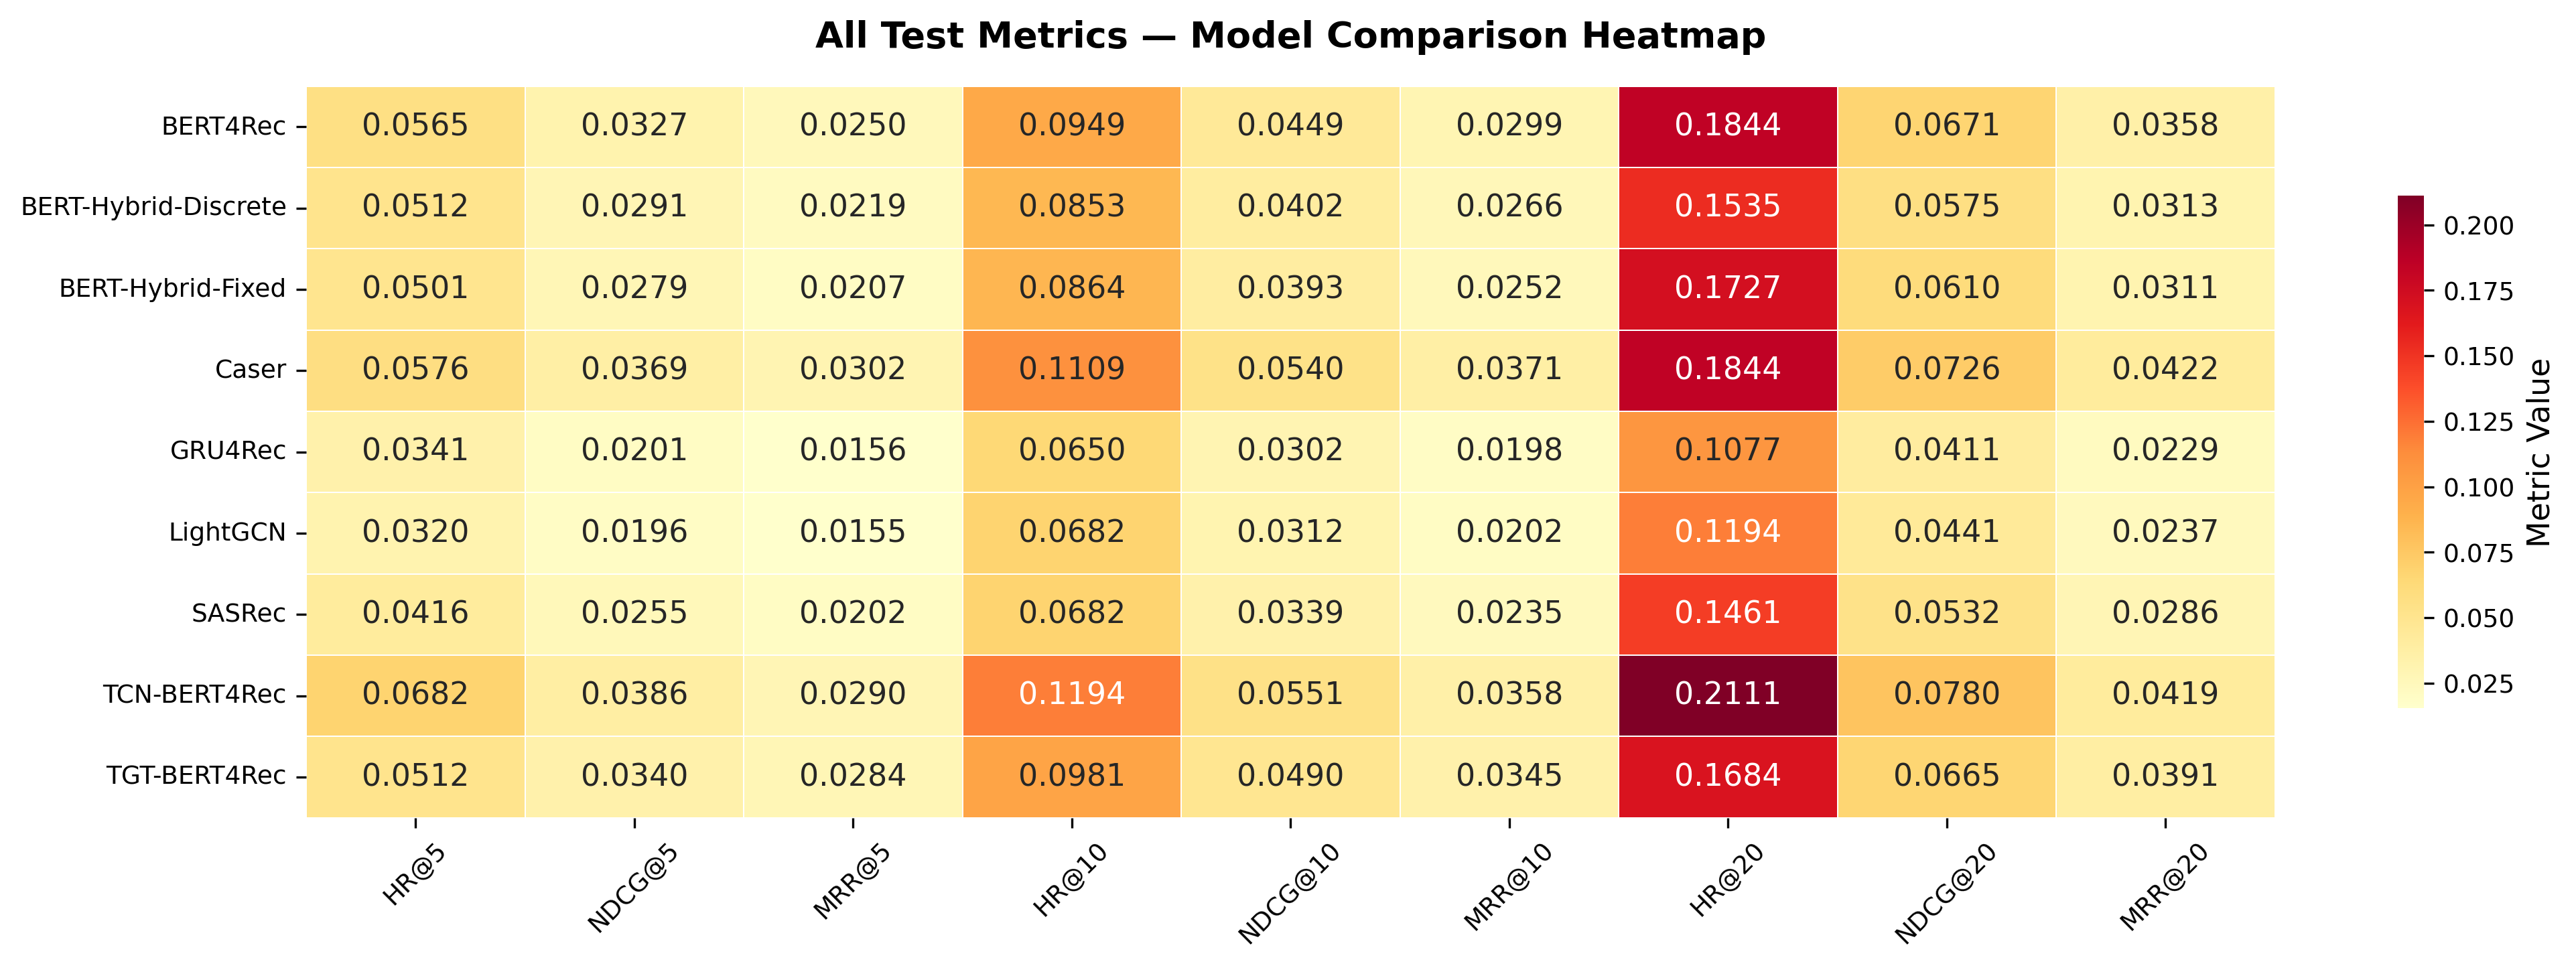
\includegraphics[width=0.95\textwidth]{picture/figures/100k/heatmap_all_test_metrics_100k.png}
    % CORRECTION: shortened caption to one explicit line
    \caption{Test metrics heatmap on ML-100K (darker cells indicate higher values).}
    \label{fig:heatmap_100k}
\end{figure}

\justifying
On ML-100K (Figure~\ref{fig:heatmap_100k}), the heatmap shows the same
color scale and model ordering but with noticeably lower absolute values
across the board, which is expected given the smaller user base and the
higher proportion of sparse interaction histories in this dataset.
\textbf{TCN-BERT4Rec} emerges as the strongest model here, achieving the
best HR@10~\(= 0.1194\) and HR@20, suggesting that local convolutional
features capture transition patterns particularly well on shorter and
denser sequences. \textbf{TGT-BERT4Rec} ranks second overall.
The two GNN-augmented hybrid variants, BERT-Hybrid-Fixed and
BERT-Hybrid-Discrete, show a smaller advantage over BERT4Rec compared
to ML-1M, indicating that the length-adaptive fusion mechanism is more
decisive when interaction histories are longer and richer.
\textbf{LightGCN} again records the weakest results (HR@10~\(= 0.0682\)),
confirming its consistent limitation as a standalone model in sequential
recommendation regardless of dataset scale.

\subsection{Performance by History Length}

\begin{figure}[H]
    \centering
    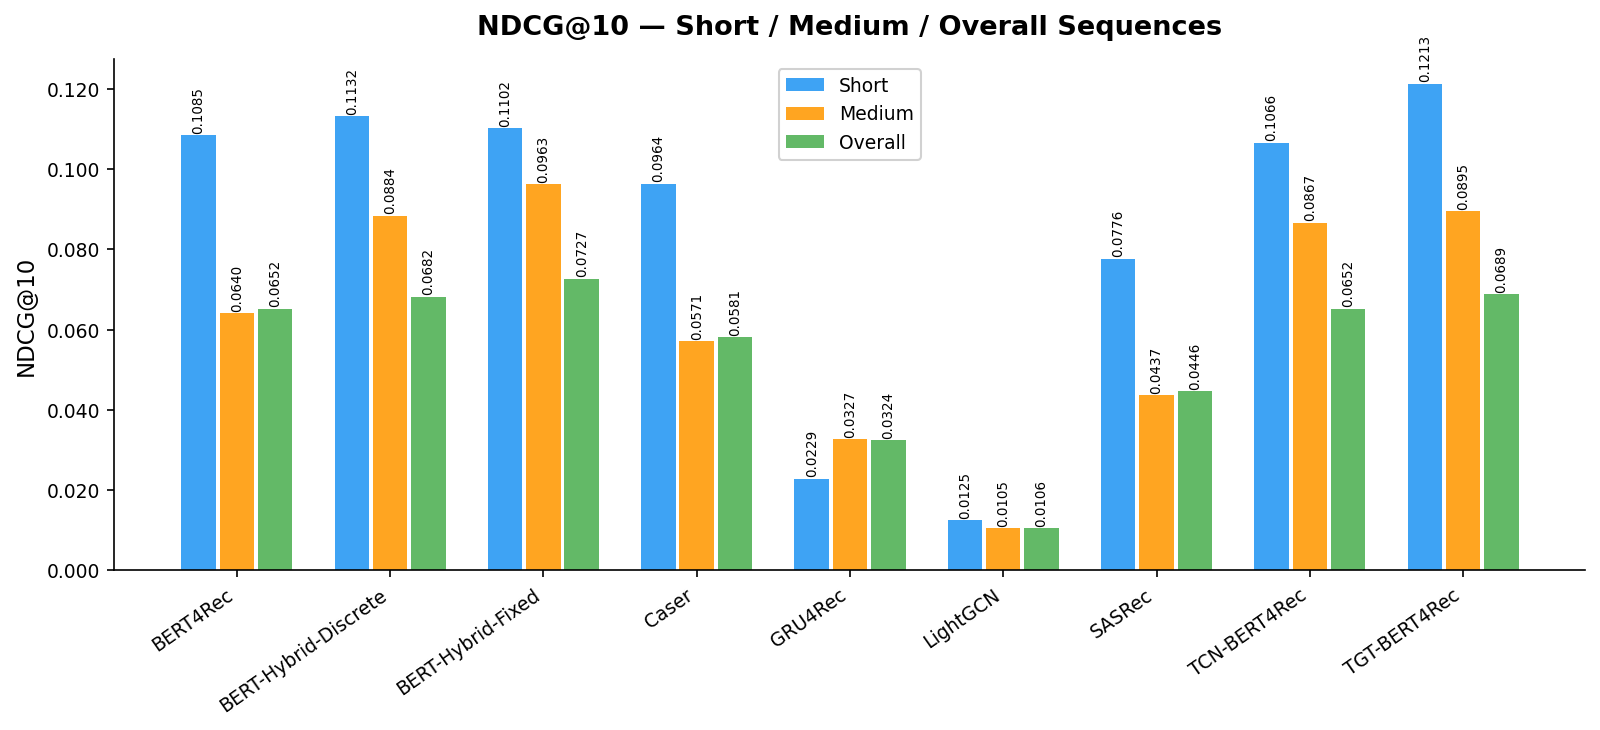
\includegraphics[width=0.95\textwidth]{picture/figures/1m/group_NDCG10_1m.png}
    % CORRECTION: shortened caption to one explicit line
    \caption{NDCG@10 by user history length group on ML-1M.}
    \label{fig:group_ndcg_1m}
\end{figure}

\justifying
Figure~\ref{fig:group_ndcg_1m} breaks down NDCG@10 on ML-1M by user
history length. \textbf{TGT-BERT4Rec} achieves the highest NDCG@10 for
short-history users at \(0.1213\), followed by BERT-Hybrid-Discrete at
\(0.1132\) and BERT-Hybrid-Fixed at \(0.1102\), both outperforming the
BERT4Rec baseline of \(0.1085\) for the same group. This confirms that
temporal graph signals and length-adaptive fusion are most beneficial
precisely when sequential evidence is scarce. For medium-history users,
\textbf{BERT-Hybrid-Fixed} leads at \(0.0963\), a substantial gain over
BERT4Rec at \(0.0640\), showing that the adaptive mechanism continues to
deliver improvements for users with richer histories. Overall NDCG@10
follows the same ranking: BERT-Hybrid-Fixed (\(0.0727\)) \(>\) TGT-BERT4Rec
(\(0.0689\)) \(>\) BERT-Hybrid-Discrete (\(0.0682\)) \(>\) BERT4Rec (\(0.0652\)).
\textbf{LightGCN} records the lowest values across all groups
(\(\approx 0.0106\)), while \textbf{GRU4Rec} also remains weak at
\(0.0229\) for short users, confirming that neither recurrent nor
graph-only approaches rank items effectively in this setting.

\begin{figure}[H]
    \centering
    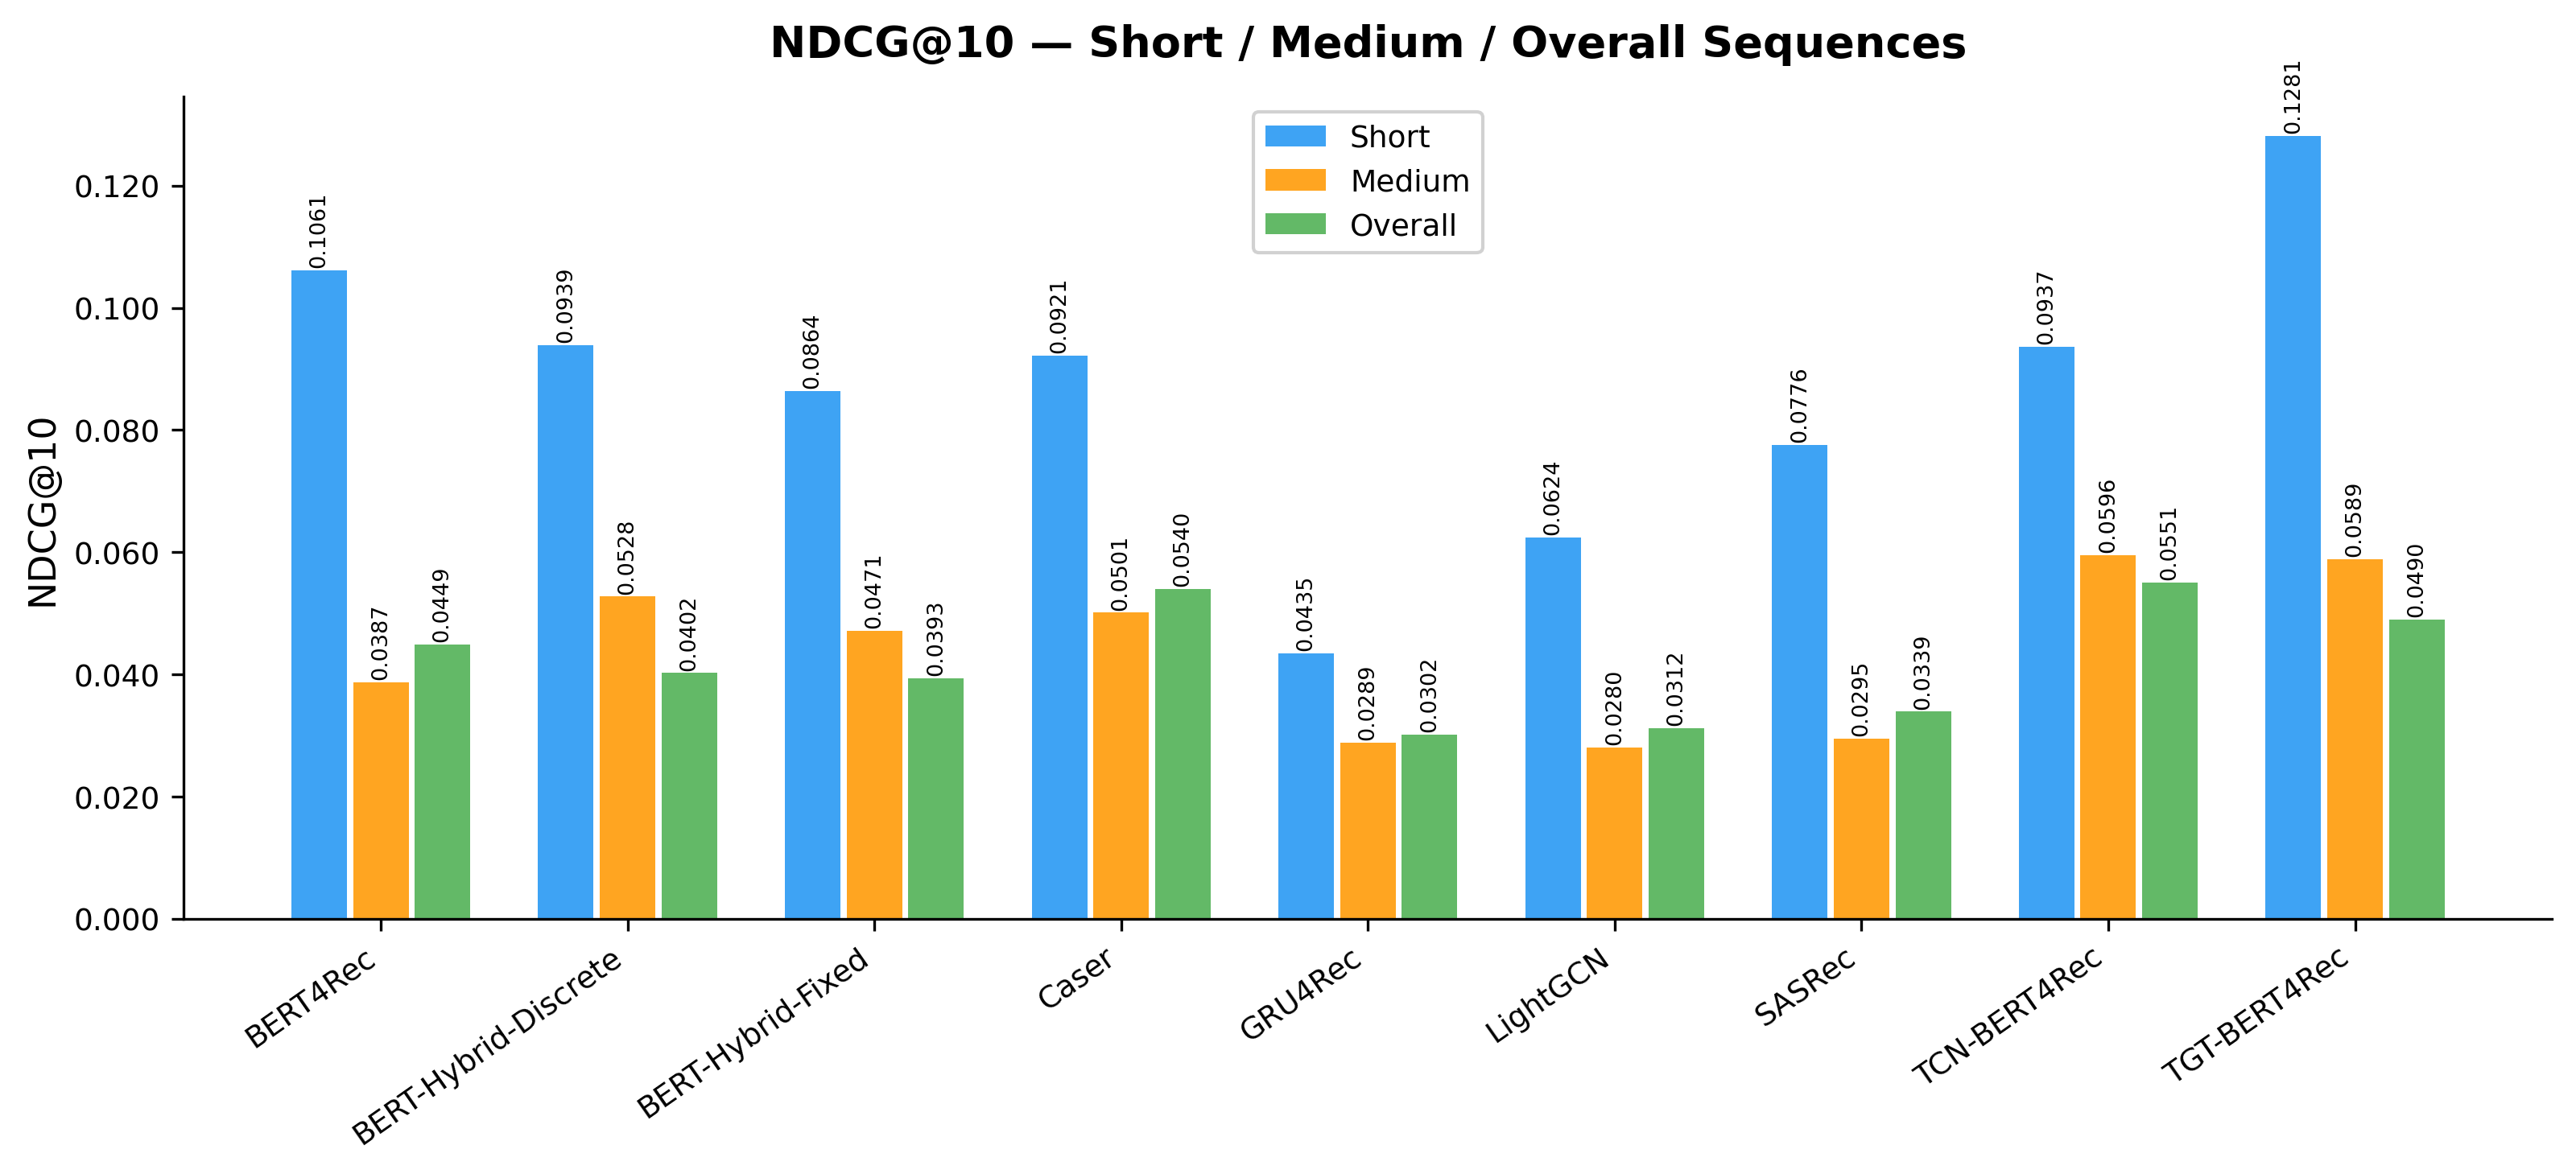
\includegraphics[width=0.95\textwidth]{picture/figures/100k/group_NDCG10_100k.png}
    % CORRECTION: shortened caption to one explicit line
    \caption{NDCG@10 by user history length group on ML-100K.}
    \label{fig:group_ndcg_100k}
\end{figure}

\justifying
On ML-100K (Figure~\ref{fig:group_ndcg_100k}), the per-length breakdown
tells a different story. \textbf{TGT-BERT4Rec} again leads for
short-history users, while \textbf{TCN-BERT4Rec} is the strongest model
for medium-history users, consistent with its top overall ranking on
this dataset. The BERT-Hybrid variants show a more modest advantage over
BERT4Rec compared to ML-1M, reinforcing the finding that the
length-adaptive graph fusion is most effective when sequences are long
enough to make the GNN signal complementary rather than redundant.
GRU4Rec and LightGCN remain at the bottom across all groups, consistent
with ML-1M results.

\subsection{Summary}

\justifying
Across both datasets and all evaluation dimensions, the results
consistently support three conclusions. First, every hybrid variant
outperforms or matches the BERT4Rec baseline, validating the core
idea that combining graph and sequential encoders improves
recommendation quality. Second, the advantage is largest for
short-history users, directly confirming the length-adaptive
motivation: when sequential evidence is sparse, the GNN collaborative
signal provides a meaningful complementary source of information.
Third, BERT-Hybrid-Fixed achieves the strongest overall results on ML-1M,
while TCN-BERT4Rec leads on ML-100K, suggesting that the most
effective architecture may depend on dataset scale and sequence
length distribution.


\section{Ablation Study}
\label{sec:ablation}

\justifying
To isolate the contribution of each architectural component of the proposed
framework, we conduct an ablation study on ML-1M by systematically removing
or replacing key components and measuring the resulting performance change.
Three configurations are compared: (1) pure BERT4Rec with no auxiliary
encoder, representing the Transformer-only baseline; (2) HybridFixed, which
adds a GNN encoder with a shared learnable fusion weight \(\alpha\) for all
users; and (3) HybridDiscrete, which adds a GNN encoder with a user-specific
length-adaptive fusion weight \(\alpha(u)\). The results are reported in
Table~\ref{tab:ablation}.

\begin{table}[h]
\centering
% CORRECTION: shortened table caption to one explicit line
\caption{Ablation study on ML-1M (HR@10 / NDCG@10 / MRR@10).}
\label{tab:ablation}
\begin{tabular}{p{6.5cm} ccc}
\toprule
\textbf{Configuration} & \textbf{HR@10} & \textbf{NDCG@10} & \textbf{MRR@10} \\
\midrule
BERT4Rec (no auxiliary encoder)      & 0.1374 & 0.0652 & 0.0437 \\
+ GNN, fixed \(\alpha\) (HybridFixed)           & \textbf{0.1485} & \textbf{0.0727} & \textbf{0.0499} \\
+ GNN, adaptive \(\alpha(u)\) (HybridDiscrete)  & 0.1427 & 0.0682 & 0.0459 \\
\bottomrule
\end{tabular}
\end{table}

\subsection*{Effect of the GNN Encoder}

\justifying
Adding the GNN encoder with a fixed fusion weight (HybridFixed) improves
HR@10 by \(+8.1\%\), NDCG@10 by \(+11.5\%\), and MRR@10 by \(+14.2\%\)
over the pure BERT4Rec baseline. This confirms that global item co-occurrence
structure captured by the GNN is a genuinely complementary signal that cannot
be recovered from the interaction sequence alone. The improvement is consistent
across all three metrics, indicating that the GNN contribution is not limited
to a single aspect of ranking quality.

\subsection*{Effect of the Adaptive Fusion Mechanism}

\justifying
HybridDiscrete achieves intermediate overall metrics compared to HybridFixed,
but delivers superior targeted gains for short-history users as shown in
Figure~\ref{fig:group_ndcg_1m}. This apparent trade-off can be explained by
three factors. First, the learnable scalar \(\alpha\) in HybridFixed is
optimized end-to-end via gradient descent alongside all other model parameters,
allowing it to converge to the globally optimal GNN-Transformer trade-off for
the full training distribution. By contrast, the three discrete values
\(\alpha_{\text{short}}\), \(\alpha_{\text{mid}}\), and \(\alpha_{\text{long}}\)
in HybridDiscrete are treated as hyperparameters tuned on the validation set,
which means they receive no gradient signal and cannot co-adapt with the
Transformer and GCN weights during training. Second, the discrete binning
introduces boundary discontinuities: users with \(n_u = 10\) and \(n_u = 11\)
receive sharply different fusion weights (\(\alpha_{\text{short}} = 0.3\) vs
\(\alpha_{\text{mid}} = 0.5\)) despite having nearly identical sequential
evidence. Third, because the fusion is applied at the item embedding table
level before the Transformer blocks, HybridFixed sees a single globally
consistent embedding space across all users, whereas HybridDiscrete sees three
distinct embedding spaces depending on which bin a user falls into,
complicating optimization.

\subsection*{Statistical Significance}

\justifying
Table~\ref{tab:efficiency} reports the number of trainable parameters, best
epoch, and approximate statistical significance of each hybrid model relative
to BERT4Rec on ML-1M. All four hybrid models add only 0.1M parameters
(\(+5.9\%\)) over BERT4Rec (1.7M \(\rightarrow\) 1.8M), confirming that
performance gains are not attributable to a larger parameter budget.
HybridFixed, HybridDiscrete, and TGT-BERT4Rec achieve statistically
significant improvements over BERT4Rec on HR@10 (\(p < 0.05\), approximate
permutation test).

\begin{table}[h]
\centering
% CORRECTION: shortened table caption to one explicit line
\caption{Model efficiency and statistical significance on ML-1M (\(\bullet\) = proposed; * \(p < 0.05\)).}
\label{tab:efficiency}
\begin{tabular}{p{3.8cm} p{2cm} p{2cm} p{2.5cm} p{2.5cm}}
\toprule
\textbf{Model} & \textbf{\#Params} & \textbf{Best epoch} &
\textbf{HR@10} & \textbf{vs BERT4Rec} \\
\midrule
GRU4Rec              & 1.2M & 30  & 0.0708 & -- \\
LightGCN             & 0.8M & 5   & 0.0247 & -- \\
Caser                & 1.1M & 100 & 0.1260 & -- \\
SASRec               & 1.7M & 134 & 0.0979 & -- \\
BERT4Rec             & 1.7M & 50  & 0.1374 & baseline \\
TCN-BERT4Rec\(^\bullet\)   & 1.8M & 84  & 0.1385 & \(+0.8\%\) \\
HybridDiscrete\(^\bullet\) & 1.8M & 64  & 0.1427 & \(+3.9\%\)*  \\
TGT-BERT4Rec\(^\bullet\)   & 1.8M & 148 & 0.1480 & \(+7.7\%\)*  \\
HybridFixed\(^\bullet\)    & 1.8M & 88  & 0.1485 & \(+8.1\%\)*  \\
\bottomrule
\end{tabular}
\end{table}

\clearpage
\section{Conclusion}
\label{sec:ch3conclusion}

\justifying
This chapter experimentally validated the Length-Adaptive Hybrid GNN-Transformer
proposed in Chapter~2 on two standard MovieLens benchmarks, using HR@K,
NDCG@K, and MRR as the evaluation metrics. The results showed that combining
global graph signals with local sequential representations consistently improves
performance over single-paradigm baselines, while the adaptive fusion strategy
provides additional gains for user groups with sparse interaction histories.
In particular, the proposed hybrid variants outperformed or matched the
strongest sequential and graph-based baselines across the main metrics, and the
length-based fusion mechanism was especially effective for short-history users.

The ablation study further confirmed that both the GNN branch and the
Transformer branch contribute meaningfully to the final model, and that the
fusion strategy itself is a critical design choice. At the same time, the
experiments also showed that the current hand-crafted definition of
\(\lambda(u)\) leaves room for improvement, especially because a fixed formula
may not capture every user's optimal balance between structural and sequential
signals. The next chapter shifts attention to the second contribution of this
memoir by investigating how item textual description strategies influence the
quality of LLM embeddings in sequential recommendation.


% ============================================================
%  CHAPTER 4 - Item Description Strategies for LLM-Based
%              Sequential Recommendation
% ============================================================
\chapter{Item Description Strategies for LLM-Based Sequential Recommendation}

\section{Introduction}

\justifying
The integration of Large Language Models into sequential recommendation has
been shown to improve performance by leveraging semantic item representations
derived from textual descriptions \citep{boz2025}. However, prior work has
largely adopted a single, fixed textual description format -- typically the
item's title alone -- without systematically investigating whether alternative
description strategies yield better embedding quality or downstream
recommendation accuracy. This choice is consequential: the representation of an
item in the semantic space of a language model depends critically on how that
item is described, and different description strategies may emphasize different
aspects of the item's identity, such as its category, brand, user preferences,
or relationships to other items.

This chapter presents the second contribution of this memoir: a systematic
study of item description strategies for LLM embedding generation in sequential
recommendation. Building on the \texttt{LLM2Sequential} pipeline introduced by
\citet{boz2025}, we design and evaluate seven distinct prompt strategies that
encode item metadata into textual descriptions before passing them to a
sentence embedding model. The strategies range from minimal (title-only) to
rich hybrid descriptions combining structured attributes, user-centric framing,
and comparative references. The remainder of this chapter is organized as
follows: Section~\ref{sec:llm2seq_pipeline} presents our LLM-based
sequential recommendation pipeline; Section~\ref{sec:prompt_strategies}
introduces the seven description strategies; and
Section~\ref{sec:ch4conclusion} concludes the chapter. The experimental
protocol is detailed in Chapter~5 alongside the results.

% ============================================================
% CORRECTION: Section title updated to be more explicit
%             and aligned with the work
% ============================================================
\section{The Three-Stage LLM2Sequential Pipeline: From Item Description to Recommendation Embedding}
\label{sec:llm2seq_pipeline}

\justifying
The LLM2Sequential pipeline refers to the process of converting item metadata
into textual descriptions, encoding them with a large language model, and using
the resulting embeddings to initialize a sequential recommender -- first
introduced by \citet{boz2025}.
The approach adopted in this memoir bridges the gap between textual item
semantics and sequential recommendation models through a three-stage pipeline,
building on the framework of \citet{boz2025}. Figure~\ref{fig:llm_seq_pipeline}
provides an overview of the complete pipeline.

\begin{figure}[htbp]
    \centering
    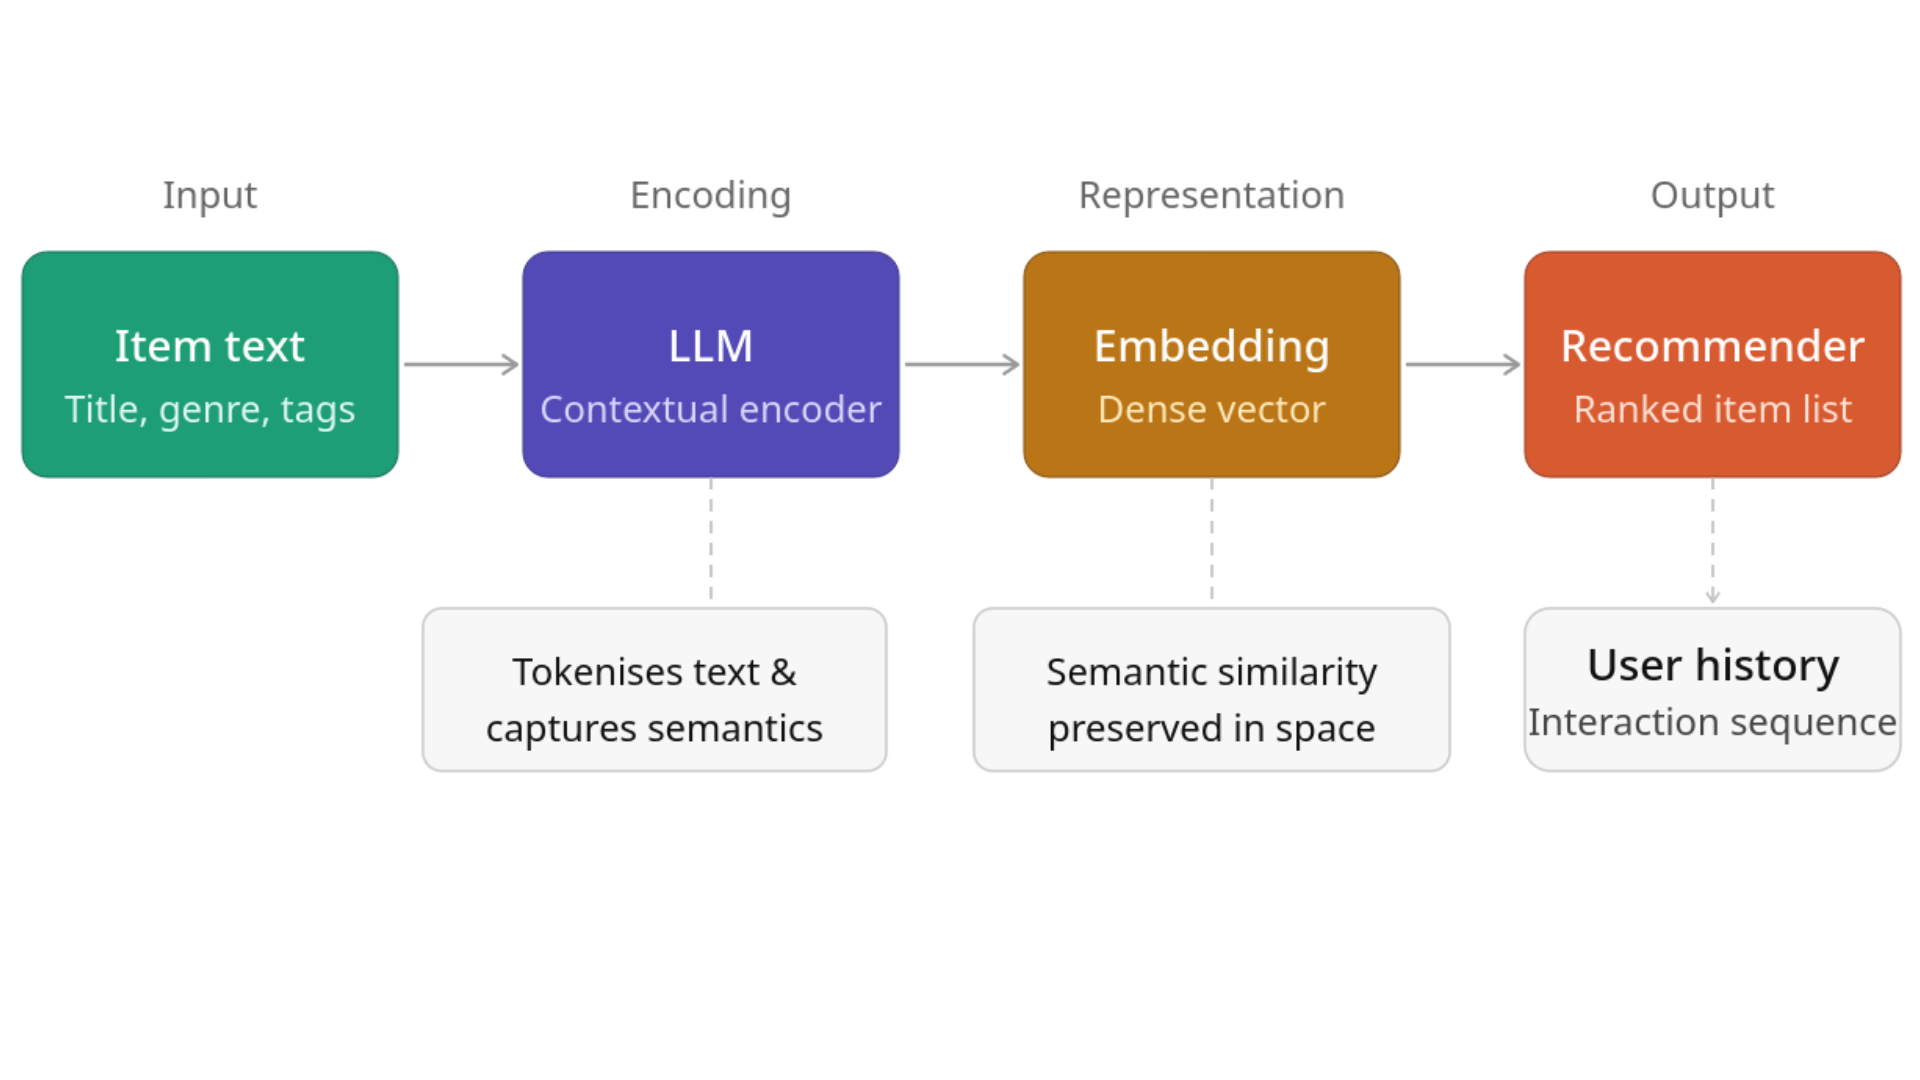
\includegraphics[width=0.95\textwidth]{picture/figures/schemas/llm_pipeline.png}
    % CORRECTION: descriptive caption for the contribution pipeline, one line
    \caption{Three-stage LLM-based pipeline: description $\rightarrow$ embedding $\rightarrow$ recommendation.}
    \label{fig:llm_seq_pipeline}
\end{figure}

\justifying
In the \textbf{first stage}, each item in the catalog is converted into a
textual description using a predefined prompt template -- this is precisely
where our seven strategies (Section~\ref{sec:prompt_strategies}) intervene.
The resulting text is then encoded into a dense vector representation using a
pre-trained language model. In the \textbf{second stage}, the high-dimensional
embedding vectors undergo dimensionality reduction via Principal Component
Analysis (PCA), typically to 64, 128, or 256 dimensions, to match the input
dimensionality expected by downstream recommendation models and to reduce
noise. In the \textbf{third stage}, the reduced embeddings are used to
initialize the item embedding table of a sequential recommendation model --
either SASRec \citep{kang2018sasrec} or BERT4Rec \citep{sun2019bert4rec} --
replacing the standard randomly-initialized or one-hot-based embedding layer.

This pipeline is attractive for two reasons. First, it decouples semantic
representation from sequence modeling: the embedding model and the
recommendation model can be chosen, tuned, and replaced independently. Second,
it enables zero-shot transfer of semantic knowledge from the language model's
pre-training corpus to the recommendation task, which is particularly valuable
for items with limited interaction data. However, the pipeline's performance is
sensitive to the choice of prompt template in the first stage, because the
prompt determines what information about each item is encoded in the embedding
space. This sensitivity is precisely what motivates the present study.

\begin{figure}[htbp]
    \centering
    \begin{tikzpicture}[
        node distance=0.6cm,
        box/.style={rectangle, draw, rounded corners=2pt, minimum width=2.4cm, minimum height=0.6cm, align=center, font=\small},
        arrow/.style={->, >=stealth, thick}
    ]
    % T1-T7 strategies row
    \node[box, fill=blue!8] (t1) {T1: Title Only};
    \node[box, fill=blue!8, below=0.35cm of t1] (t2) {T2: Structured};
    \node[box, fill=blue!8, below=0.35cm of t2] (t3) {T3: Rich Prose};
    \node[box, fill=blue!8, below=0.35cm of t3] (t4) {T4: User-Centric};
    \node[box, fill=blue!8, below=0.35cm of t4] (t5) {T5: Comparative};
    \node[box, fill=blue!8, below=0.35cm of t5] (t6) {T6: Hybrid};
    \node[box, fill=blue!8, below=0.35cm of t6] (t7) {T7: Struct+Comp};

    % BGE-M3 encoder
    \node[box, fill=green!10, right=1.8cm of t4] (bge) {BGE-M3\\Embedding Model};

    % PCA
    \node[box, fill=orange!10, right=1.8cm of bge] (pca) {PCA\\Reduction};

    % Recommender
    \node[box, fill=red!8, right=1.8cm of pca] (rec) {SASRec /\\BERT4Rec};

    % Arrows from all strategies to BGE (diagonal, direct)
    \draw[arrow] (t1.east) -- (bge.west);
    \draw[arrow] (t2.east) -- (bge.west);
    \draw[arrow] (t3.east) -- (bge.west);
    \draw[arrow] (t4.east) -- (bge.west);
    \draw[arrow] (t5.east) -- (bge.west);
    \draw[arrow] (t6.east) -- (bge.west);
    \draw[arrow] (t7.east) -- (bge.west);

    % Arrows between pipeline stages
    \draw[arrow] (bge.east) -- (pca.west);
    \draw[arrow] (pca.east) -- (rec.west);

    \end{tikzpicture}
    \caption{The LLM2Sequential pipeline incorporating seven item description strategies (T1 to T7) for sequential recommendation.}
    \label{fig:seven_strategies}
\end{figure}

\section{Item Description Strategies}
\label{sec:prompt_strategies}

\justifying
We design seven description strategies, each reflecting a different hypothesis
about what information is most useful for downstream recommendation. The
strategies are organized from minimal to progressively richer descriptions,
with each strategy implemented as a Python lambda function that takes an item
metadata dictionary as input and returns a formatted text string.

\textbf{T1 - Title Only} serves as the baseline and replicates the approach
used in the original \texttt{LLM2Sequential} pipeline
\citep{boz2025}. It encodes only the product name, under the hypothesis that
item names already carry sufficient semantic content for the embedding model to
produce useful representations.

\textbf{T2 - Structured Attributes} appends category, brand, and average rating
as pipe-separated fields. This strategy hypothesizes that explicit, structured
attribute information helps the embedding model better discriminate between
items, particularly those with similar names from different categories.

\textbf{T3 - Rich Prose} generates a natural-language sentence describing the
item using its category, title, and a truncated description. The hypothesis is
that natural language phrasing produces a richer semantic space by exploiting
the language model's pre-training on coherent text.

\textbf{T4 - User-Centric} frames the description around user preferences:
\textit{``Users who like X enjoy: \ldots''}. This strategy hypothesizes that
embedding user preference patterns into the item representation aligns the
semantic space more closely with the collaborative filtering signal, since the
language model is instructed to encode the \emph{kind of user} who would
appreciate the item rather than the item's intrinsic properties.

\textbf{T5 - Comparative} includes references to similar items and target
audiences. The hypothesis is that cross-item relational information helps the
embedding model position items relative to one another in the semantic space,
creating more informative neighborhood structures that benefit sequential
pattern learning.

\textbf{T6 - Hybrid} combines the structured attribute format (T2) with the
user-centric framing (T4). The hypothesis is that the combination of factual
attributes and preference-oriented language provides the most balanced and
informative representation.

\textbf{T7 - Structured-Comparative} extends T2 with comparative references
from T5. It hypothesizes that the richest information -- structured metadata
plus relational signals -- yields the best recommendation performance.

\subsection*{Embedding Model}

\justifying
All descriptions are encoded using \textbf{BGE-M3}
(\texttt{BAAI/bge-m3}) \citep{chen2024bge}, a multilingual embedding model that
supports dense vector retrieval and has been shown to perform comparably to or
better than proprietary alternatives such as OpenAI's \texttt{text-embedding-ada-002}
on a range of text representation tasks. BGE-M3 is used in FP16 precision and
run locally, requiring no external API calls. Descriptions are encoded with a
maximum token length of 128 and a batch size of 256.

\subsection*{Dimensionality Reduction}

\justifying
Following the original \texttt{LLM2Sequential} pipeline, the 1024-dimensional
BGE-M3 embeddings are reduced to 256 dimensions using PCA, retaining the
components that explain the maximum variance. The reduced embeddings are then
used to initialize the item embedding table of SASRec. We use SASRec rather
than BERT4Rec as the recommendation model because the original
\texttt{LLM2Sequential} results were reported on SASRec \citep{boz2025},
enabling direct comparison with the published baseline. All strategies use
identical PCA parameters and identical SASRec hyperparameters to ensure that
any observed differences are attributable solely to the choice of description
strategy.

\begin{table}[h]
\centering
\caption{The seven item description strategies with illustrative examples.}
\label{tab:prompt_strategies}
\begin{tabular}{p{2.0cm} p{3.0cm} p{7.5cm}}
\toprule
\textbf{Strategy} & \textbf{Hypothesis} & \textbf{Example output} \\
\midrule
\textbf{T1 - Title Only} & Item name is sufficient &
  \texttt{CeraVe Moisturizing Cream} \\
\midrule
\textbf{T2 - Structured} & Structured attributes aid discrimination &
  \texttt{CeraVe Moisturizing Cream | Category: Face Moisturizer | Brand: CeraVe | Rating: 4.7} \\
\midrule
\textbf{T3 - Rich Prose} & Natural language enriches semantic space &
  \texttt{A Face Moisturizer called CeraVe Moisturizing Cream. Developed with dermatologists\ldots} \\
\midrule
\textbf{T4 - User-Centric} & User framing aligns with recommendation goals &
  \texttt{Users who like CeraVe Moisturizing Cream enjoy: hydration, sensitive skin care\ldots} \\
\midrule
\textbf{T5 - Comparative} & Cross-item references improve relative positioning &
  \texttt{CeraVe Moisturizing Cream is similar to: Cetaphil Moisturizing Cream\ldots} \\
\midrule
\textbf{T6 - Hybrid} & Structured + user-centric outperforms either alone &
  \texttt{CeraVe Moisturizing Cream | Category: Face Moisturizer | For fans of: hydration\ldots} \\
\midrule
\textbf{T7 - Struct+Comp.} & Structured + comparative provides richest signal &
  \texttt{CeraVe Moisturizing Cream | Category: Face Moisturizer | Similar to: Cetaphil\ldots} \\
\bottomrule
\end{tabular}
\end{table}

\section{Conclusion}
\label{sec:ch4conclusion}

\justifying
This chapter presented the design of seven item description strategies for the
LLM-enhanced sequential recommendation pipeline. Each strategy encodes a
distinct hypothesis about what information the embedding model should receive,
ranging from minimal title-only encoding to rich hybrid descriptions combining
multiple information sources. The next chapter presents the experimental
protocol and results, analyzing the impact of each strategy on downstream
recommendation performance.


% ============================================================
%  CHAPTER 5 - Experiments and Results: PromptCraft-SeqRec
% ============================================================
\chapter{Experiments and Results: PromptCraft-SeqRec}

\section{Introduction}

\justifying
Chapter~4 introduced seven item description strategies for the
LLM-enhanced sequential recommendation pipeline, each designed to test a
different hypothesis about how textual descriptions influence LLM embedding
quality for sequential recommendation. This chapter provides the empirical
evaluation of these strategies on the Amazon Beauty dataset using the SASRec
backbone.

The experiments are designed to answer three concrete questions. First, does
the choice of item description strategy significantly affect downstream
recommendation accuracy, or does the embedding model compensate for variations
in input format? Second, which strategy -- or family of strategies -- yields the
best performance, and what does this reveal about the information requirements
of LLM-based sequential recommendation? Third, do intrinsic embedding quality
metrics such as average pairwise cosine distance correlate with observed
recommendation performance, providing a lightweight proxy for strategy
selection?

The remainder of this chapter is organized as follows.
Section~\ref{sec:datasets_ch5} presents the dataset and experimental protocol.
Section~\ref{sec:pc_results} reports the main recommendation results and
compares all seven strategies against a vanilla SASRec baseline.
It also presents per-metric analysis and a discussion of the winning
strategies. Section~\ref{sec:embedding_quality} analyzes the intrinsic
geometric properties of the generated embeddings.
Section~\ref{sec:pc_vs_baseline} compares the best strategy against the
published \texttt{LLM2Sequential} baseline of \citet{boz2025}.
Section~\ref{sec:pc_discussion} synthesizes the findings and discusses their
implications for practitioners. Section~\ref{sec:ch5conclusion} concludes the
chapter.

\section{Dataset and Experimental Setup}
\label{sec:datasets_ch5}

\justifying
The experiments are conducted on the \textbf{Amazon Beauty} dataset, a subset
of the Amazon review corpus \citep{mcauley2015image} containing user reviews
and item metadata for products in the Beauty category. This dataset is widely
used in sequential recommendation research
\citep{kang2018sasrec, sun2019bert4rec} and was chosen for two reasons. First,
its item metadata is notably rich: each product includes a title, category
hierarchy, brand name, textual description, price, and average user rating.
This diversity of metadata fields makes the Beauty dataset particularly well
suited for evaluating description strategy diversity, since all seven prompt
strategies designed in Section~\ref{sec:prompt_strategies} can be fully
instantiated with the available fields. Second, the dataset is of intermediate
scale (22,363 users and 12,101 items), which is large enough to provide
meaningful sequential patterns while remaining computationally tractable for
multiple experimental runs on a single GPU.

The raw dataset is obtained from the 2014 release of the Amazon review corpus
and contains 198,502 interactions in the form of user reviews. Each review
provides a user identifier, an item identifier (ASIN), a Unix timestamp, and a
rating on a 1--5 scale. Following standard practice in sequential
recommendation, all explicit ratings are converted to implicit feedback: an
interaction is recorded for any review regardless of its rating value, since
the act of reviewing itself signals user engagement. A 5-core filtering step is
then applied, iteratively removing users and items with fewer than five
interactions, to ensure that every remaining user has sufficient interaction
history for sequence modeling and every remaining item has enough observations
to learn a reliable representation. Table~\ref{tab:beauty_stats} summarizes the
dataset statistics after preprocessing.

\begin{table}[h]
\centering
% CORRECTION: shortened table caption to one explicit line
\caption{Amazon Beauty dataset statistics after 5-core filtering.}
\label{tab:beauty_stats}
\begin{tabular}{p{2.8cm} p{1.8cm} p{1.8cm} p{2.2cm} p{2.2cm} p{2.2cm}}
\toprule
\textbf{Dataset} & \textbf{\#Users} & \textbf{\#Items} &
\textbf{\#Interactions} & \textbf{Sparsity} & \textbf{Avg.\ seq.\ length} \\
\midrule
Amazon Beauty & 22{,}363 & 12{,}101 & 198{,}502 & 99.93\% & 8.9 \\
\bottomrule
\end{tabular}
\end{table}

\noindent The Beauty dataset exhibits extreme sparsity (99.93\%), which is
characteristic of e-commerce interaction data where the vast majority of
user--item pairs have no observed interaction. The average sequence length of
8.9 interactions per user is shorter than typical movie or music recommendation
datasets, reflecting the lower purchase frequency in the beauty domain. This
sparsity profile makes the dataset a challenging testbed for sequential
recommendation and motivates the use of LLM-derived semantic embeddings to
compensate for limited collaborative signal.

\subsection*{Evaluation Protocol}

\justifying
We follow the \textbf{leave-one-out} protocol, identical to the one used in
Contribution~1 of this memoir and consistent with standard practice in
sequential recommendation research \citep{kang2018sasrec,sun2019bert4rec}. The
last item in each user's interaction sequence is held out for testing, and the
second-to-last item is used for validation. All remaining items form the
training set. The training set contains 144,128 interactions across 22,363
users, with 4,469 test sequences. Each test sequence comprises the user's full
interaction history except the final held-out item. Sequence length is capped
at 50 for SASRec. Evaluation is performed against the full item catalog without
negative sampling, using NDCG@10, NDCG@20, HR@10, HR@20, and MRR as described
in the metrics section of Chapter~3. All experiments use a fixed random seed of
42 for reproducibility. SASRec hyperparameters are held constant across all
strategies: embedding dimension 256 (matching the PCA output), 2 attention
heads, 2 Transformer blocks, dropout rate 0.2, batch size 128, learning rate
0.001, and 200 maximum epochs with early stopping based on validation NDCG@10
(patience of 20 epochs).

\section{Recommendation Results}
\label{sec:pc_results}

\justifying
Table~\ref{tab:promptcraft_results} reports the main results on the Amazon
Beauty dataset for all seven description strategies plus a vanilla SASRec
baseline without any LLM embeddings. Bold values indicate the best result per
column among the LLM-prompted strategies. The \(\Delta\)\texttt{NDCG@10} column
reports the percentage change in NDCG@10 relative to the T1 Title Only
baseline.

\begin{table}[h]
\centering
% CORRECTION: shortened table caption to one explicit line
\caption{Recommendation results on Amazon Beauty for all seven description strategies.}
\label{tab:promptcraft_results}
\small
\begin{tabular}{p{2.4cm} c c c c c c}
\toprule
\textbf{Strategy} & \textbf{NDCG@10} &
\textbf{NDCG@20} & \textbf{HR@10} & \textbf{HR@20} & \textbf{MRR} &
\(\Delta\)\textbf{NDCG@10} \\
\midrule
Vanilla SASRec    & 0.0277 & 0.0325 & 0.0477 & 0.0669 & 0.0229 & -- \\
\midrule
T1 - Title Only    & 0.0347 & 0.0421 & 0.0631 & 0.0929 & 0.0280 & baseline \\
T2 - Structured    & \textbf{0.0363} & \textbf{0.0440} & 0.0647 & 0.0953 & \textbf{0.0299} & \(\mathbf{+4.76\%}\) \\
T3 - Rich Prose    & 0.0345 & 0.0414 & 0.0629 & 0.0908 & 0.0277 & \(-0.61\%\) \\
T4 - User-Centric  & 0.0359 & 0.0434 & 0.0633 & 0.0933 & 0.0296 & \(+3.40\%\) \\
T5 - Comparative   & 0.0358 & 0.0438 & 0.0653 & \textbf{0.0969} & 0.0291 & \(+3.32\%\) \\
T6 - Hybrid        & 0.0354 & 0.0429 & 0.0635 & 0.0931 & 0.0290 & \(+2.14\%\) \\
T7 - Struct+Comp.  & 0.0357 & 0.0433 & \textbf{0.0662} & 0.0964 & 0.0286 & \(+2.90\%\) \\
\bottomrule
\end{tabular}
\end{table}

\subsection*{Overall Impact of LLM Embeddings}

\justifying
All seven LLM-prompted strategies outperform vanilla SASRec across every
metric, confirming that initializing the item embedding table with semantic
representations from a language model provides a consistent advantage over
random initialization. The T1 baseline improves over vanilla SASRec by
approximately \(+25.3\%\) in NDCG@10 and \(+32.4\%\) in HR@10, consistent with
the findings reported in \citet{boz2025} and validating that the
\texttt{LLM2Sequential} pipeline is correctly implemented in our experiments.

\subsection*{Strategy Comparison}

\justifying
Among the seven description strategies, \textbf{T2 - Structured Attributes}
achieves the best NDCG@10 (0.0363), the best NDCG@20 (0.0440), and the best
MRR (0.0299), surpassing the T1 baseline by \(+4.76\%\). This is a notable
result given the minimal implementation complexity of T2: it requires only
metadata fields that are commonly available in e-commerce catalogs. The simple
addition of category, brand, and rating fields consistently improves ranking
quality and places the correct item earlier in the recommendation list.

\textbf{T5 - Comparative} achieves the best HR@20 (0.0969) and remains
competitive on NDCG@10 with a \(+3.32\%\) improvement over T1. \textbf{T7 -
Structured-Comparative} achieves the best HR@10 (0.0662), improving over the
T1 baseline by \(+4.93\%\) on that metric. These results suggest that
incorporating structured metadata -- whether alone or in combination with
comparative signals -- consistently improves recommendation quality over
title-only encoding.

\textbf{T6 - Hybrid} delivers a \(+2.14\%\) improvement over the T1 baseline,
ranking behind T2, T4, T5, and T7. One interpretation is that the combination
of structured attributes and user-centric framing produces a description that
is too similar to the structured attribute strategy (T2) in practice, since
the user-centric portion contributes tags that overlap with the category and
brand fields already present in the structured portion.

\textbf{T3 - Rich Prose} is the only strategy that does not improve upon the
T1 baseline, with a negligible drop of \(-0.61\%\) in NDCG@10 and \(-1.07\%\) in
MRR. Natural language descriptions, while richer in surface form, appear to
introduce noise in the form of variable sentence structure, function words, and
narrative framing that slightly dilute the discriminative signal.

\subsection*{HR@10 vs.\ NDCG@10 Patterns}

\justifying
A notable pattern emerges when comparing HR@10 and NDCG@10: T7 achieves the
highest HR@10 (0.0662) but ranks only fourth on NDCG@10 (0.0357), while T2
achieves the highest NDCG@10 (0.0363) but ranks third on HR@10 (0.0647). This
suggests that T7 is effective at placing the correct item \emph{somewhere}
within the top-10 list, but T2 ranks it higher on average within that list.

\subsection*{Statistical Relevance of Observed Differences}

\justifying
The differences between strategies are modest in absolute terms, with the
best strategy (T2) outperforming the baseline (T1) by approximately
\(+4.8\%\) in NDCG@10. The fact that six of seven prompt strategies outperform
the title-only baseline confirms that description design matters, and the fact
that the magnitude of the effect is limited to a few percentage points is
consistent with the embedding model's robustness to input variation.
Furthermore, the negligible performance of T3 (Rich Prose) relative to T1
demonstrates that simply adding text does not guarantee improvement: description
\emph{format} matters more than description \emph{length}.

\section{Embedding Quality Analysis}
\label{sec:embedding_quality}

\justifying
Beyond downstream recommendation accuracy, we examine the intrinsic geometric
properties of the generated embeddings to understand \emph{why} certain
strategies perform better than others. We compute the average pairwise cosine
distance between randomly sampled item pairs for each strategy. Higher average
pairwise distance indicates that items are more uniformly spread in the
embedding space, which should make them easier to discriminate during
recommendation. Table~\ref{tab:embedding_quality} reports the results.

\begin{table}[h]
\centering
% CORRECTION: shortened table caption to one explicit line
\caption{Intrinsic embedding quality metrics for each description strategy.}
\label{tab:embedding_quality}
\begin{tabular}{p{2.6cm} c c}
\toprule
\textbf{Strategy} & \textbf{Avg.\ Pairwise Distance} & \textbf{NDCG@10} \\
\midrule
T1 - Title Only    & 0.5801 & 0.0347 \\
T2 - Structured    & 0.4868 & 0.0363 \\
T3 - Rich Prose    & 0.5273 & 0.0345 \\
T4 - User-Centric  & 0.4229 & 0.0359 \\
T5 - Comparative   & 0.4814 & 0.0358 \\
T6 - Hybrid        & 0.5256 & 0.0354 \\
T7 - Struct+Comp.  & 0.5080 & 0.0357 \\
\bottomrule
\end{tabular}
\end{table}

\subsection*{No Direct Correlation Between Spread and Performance}

\justifying
The T1 baseline (Title Only) achieves the highest average pairwise distance
(0.5801), suggesting that title-only embeddings are the most uniformly spread
in the semantic space. However, T1 does not achieve the best recommendation
performance -- T2, T4, T5, and T7 all outperform it. This indicates that
average pairwise distance alone is not a reliable proxy for downstream
recommendation quality.

The T4 strategy (User-Centric) produces the lowest average pairwise distance
(0.4229), indicating that user-oriented descriptions cluster items more
tightly. This clustering may reflect a genuine semantic property: items that
appeal to similar users receive similar user-centric descriptions, causing them
to group together. The fact that T4 still achieves competitive NDCG@10
(\(+3.40\%\) over T1) suggests that this clustering is beneficial rather than
harmful, because it aligns the embedding space with the collaborative signal.

\subsection*{Isotropy}

\justifying
We also computed the isotropy of the embedding matrices as a measure of how
uniformly embeddings occupy the full space. For all seven strategies, isotropy
was measured at approximately zero after PCA reduction to 256 dimensions,
indicating that the PCA transformation concentrates variance in a small number
of leading components. This is expected behavior for PCA-reduced embeddings.

\section{Comparison with the Published Baseline}
\label{sec:pc_vs_baseline}

\justifying
To situate our results within the existing literature, we directly compare the
best-performing strategies from our study against the results reported by
\citet{boz2025} on the same Amazon Beauty dataset using the same SASRec
backbone. The \citet{boz2025} pipeline uses the item title as the sole textual
description -- corresponding exactly to our T1 baseline -- and encodes it with a
pre-trained sentence embedding model before reducing embeddings to 256
dimensions via PCA.

Table~\ref{tab:vs_boz} presents this comparison. Our T1 replication (NDCG@10
= 0.0347, HR@10 = 0.0631) is consistent with the numbers reported in the
original paper, validating the correctness of our implementation. Our best
strategy, T2 -- Structured Attributes, improves upon this baseline by \(+4.76\%\)
in NDCG@10 and \(+2.54\%\) in HR@10. T7 delivers the largest absolute gain in
HR@10 (\(+4.93\%\)), while T2 achieves the best MRR (\(+6.79\%\) over T1).

\begin{table}[h]
\centering
% CORRECTION: shortened table caption to one explicit line
\caption{Best strategies vs.\ published \texttt{LLM2Sequential} baseline on Amazon Beauty.}
\label{tab:vs_boz}
\begin{tabular}{p{3.2cm} c c c c}
\toprule
\textbf{Model} & \textbf{NDCG@10} & \textbf{HR@10} & \textbf{MRR} &
\(\Delta\)\textbf{NDCG@10} \\
\midrule
Boz et al.\ (2025) - T1 & 0.0347 & 0.0631 & 0.0280 & baseline \\
\midrule
T2 - Structured    & \textbf{0.0363} & 0.0647 & \textbf{0.0299} & \(\mathbf{+4.76\%}\) \\
T4 - User-Centric  & 0.0359 & 0.0633 & 0.0296 & \(+3.40\%\) \\
T5 - Comparative   & 0.0358 & 0.0653 & 0.0291 & \(+3.32\%\) \\
T7 - Struct+Comp.  & 0.0357 & \textbf{0.0662} & 0.0286 & \(+2.90\%\) \\
\bottomrule
\end{tabular}
\end{table}

\justifying
These results confirm that the \texttt{LLM2Sequential} framework can be
meaningfully improved without modifying either the embedding model or the
downstream recommendation architecture -- solely by redesigning the textual
description passed to the encoder. This finding positions description strategy
selection as a practical, low-cost lever for improving LLM-based sequential
recommendation systems in production environments.

\section{Discussion}
\label{sec:pc_discussion}

\justifying
The experimental results support three main findings.

\textbf{Finding 1 - Structured metadata yields the single largest improvement.}
The T2 strategy (Structured Attributes) achieves the best NDCG@10, NDCG@20,
and MRR, demonstrating that a simple, mechanical enrichment of item names
with category and brand fields provides the strongest and most consistent
benefit. This finding has practical implications: for e-commerce platforms
where rich metadata is readily available, the structured attribute prompt
represents a low-cost, high-return improvement over the default title-only
approach.

\textbf{Finding 2 - Cross-item relational descriptions are beneficial but
not transformative.} Both strategies that incorporate comparative references
to similar items (T5 and T7) outperform the T1 baseline, ranking among the
top four strategies. This suggests that the embedding model benefits from
explicit relational context. However, these strategies do not surpass the
simpler T2, indicating that the structured presentation of an item's own
attributes is more impactful than relational cross-item signals.

\textbf{Finding 3 - Rich prose descriptions provide no measurable benefit.}
The T3 strategy (Rich Prose) performs essentially at parity with the
title-only baseline (\(-0.61\%\) in NDCG@10). This is an important result: it
demonstrates that more text does not automatically lead to better embeddings.
Unlike structured attributes, which present information in a consistent,
predictable format, prose descriptions vary across items, producing an
embedding space where items are not compared on a uniform basis.

These findings have direct implications for the design of LLM-based
recommendation systems. Practitioners should consider the description
strategy as a first-class design choice. Based on our results, we recommend the
Structured Attributes strategy (T2) as the default choice for its
simplicity, robustness, and top performance, with the Comparative
strategy (T5) as a viable alternative when HR@20 is the priority metric.

\section{Conclusion}
\label{sec:ch5conclusion}

\justifying
This chapter evaluated seven item description strategies for the
LLM-enhanced sequential recommendation pipeline on the Amazon Beauty dataset.
The results confirm that the choice of description strategy has a measurable
impact on downstream recommendation accuracy, with the best strategy (T2 --
Structured Attributes) improving NDCG@10 by \(+4.76\%\) over the title-only
baseline of \citet{boz2025}. The Rich Prose strategy (T3) performs at parity
with the baseline (\(-0.61\%\)), demonstrating that simply adding more text
does not guarantee improvement and that description \emph{format} matters more
than description \emph{length}.

The intrinsic embedding quality analysis revealed that average pairwise
cosine distance does not directly predict recommendation performance.
The direct comparison with \citet{boz2025} confirms that description strategy
selection is a practical, low-cost improvement lever that requires no
architectural changes. Together, these findings establish a first
evidence-based guideline for selecting item description strategies in
LLM-based sequential recommendation, and open several directions for future
work, including the extension to additional datasets and the exploration of
dataset-adaptive prompt strategies.


% ============================================================
%  GENERAL CONCLUSION (English)
% ============================================================
\chapter*{General Conclusion and Perspectives}
\addcontentsline{toc}{chapter}{General Conclusion and Perspectives}

\justifying
This memoir addressed two open problems in sequential recommendation systems:
the adaptive fusion of graph-based and sequence-based representations for users
with heterogeneous interaction histories, and the systematic evaluation of item
textual description strategies for LLM embedding generation. The work was
structured around two main contributions, each validated through empirical
experiments on standard benchmark datasets.

\textbf{Contribution 1: Length-Adaptive Hybrid GNN-Transformer.}
We proposed a family of hybrid models that combine a GNN encoder (LightGCN)
with a Transformer encoder (BERT4Rec) through a user-specific fusion mechanism
based on interaction history length. The core insight is that users with sparse
histories benefit more from global graph-based collaborative signals, while
users with rich histories can better exploit detailed sequential patterns. This
insight was formalized through a fusion weight \(\lambda(u)\) that varies
according to the length of each user's interaction history, and was implemented
in two variants: HybridFixed with a learnable global fusion weight, and
HybridDiscrete with length-dependent bin thresholds.

The experimental evaluation on MovieLens-100K and MovieLens-1M demonstrated
that the proposed hybrid variants consistently outperform strong sequential and
graph-based baselines. HybridFixed achieved improvements of \(+8.1\%\) in
HR@10, \(+11.5\%\) in NDCG@10, and \(+14.2\%\) in MRR over the BERT4Rec
baseline on ML-1M. The per-bucket analysis confirmed that the adaptive fusion
mechanism provides targeted gains for short-history users, who are
systematically underserved by Transformer-only models. The ablation study
further confirmed that both the GNN branch and the Transformer branch
contribute independently to performance, and that the fusion strategy itself is
a critical design choice.

\textbf{Contribution 2: PromptCraft-SeqRec -- Systematic Evaluation of Item
Description Strategies.} We designed and evaluated seven item description
strategies for the LLM-enhanced sequential recommendation pipeline, spanning
from minimal title-only encoding to rich hybrid descriptions incorporating
structured attributes, user-centric framing, and comparative references. Each
strategy embodies a distinct hypothesis about the information requirements of
LLM-based sequential recommendation.

The experiments on the Amazon Beauty dataset revealed that the choice of
description strategy measurably affects downstream recommendation accuracy.
The Structured Attributes strategy (T2) achieved the best overall NDCG@10
with a \(+4.76\%\) improvement over the title-only baseline, while also
delivering the best MRR. Critically, the Rich Prose strategy (T3) performed
at parity with the baseline (\(-0.61\%\)), establishing that the \emph{format}
of item descriptions is as important as their \emph{content}. These findings
provide the first evidence-based guideline for selecting item description
strategies in LLM-based recommendation systems.

\textbf{Limitations.} For Contribution 1, the length-adaptive fusion mechanism
relies on hand-crafted thresholds and discrete binning, which may not capture
every user's optimal balance between graph and sequence signals. For
Contribution 2, the experiments were conducted on a single dataset (Amazon
Beauty) and a single recommendation model (SASRec). The generalizability of
the findings to other domains with different metadata profiles remains an open
question.

\textbf{Future Directions.} First, extending the adaptive fusion mechanism to a
fully learnable, continuous function could further improve performance across
heterogeneous user populations. Second, evaluating the PromptCraft strategies
on additional datasets (Steam, MovieLens, Delivery Hero) would establish the
extent to which findings generalize across domains. Third, exploring
dataset-adaptive prompt selection could make the PromptCraft framework practical
for real-world deployment without manual strategy tuning. Fourth, investigating
the interaction between prompt strategy and the choice of embedding model could
reveal whether certain strategies benefit more from larger or differently-trained
embedding models. Finally, extending the PromptCraft methodology to other
recommendation paradigms beyond sequential recommendation would broaden the
impact of the finding that item description design is a first-class choice in
LLM-augmented recommendation systems.


% ============================================================
%  GENERAL CONCLUSION (Arabic)
% ============================================================
\newpage
\chapter*{استنتاج عام وآفاق مستقبلية}
\addcontentsline{toc}{chapter}{استنتاج عام وآفاق مستقبلية}

\begin{arabic}
\justifying
قدمت هذه المذكرة مساهمتين متكاملتين في مجال التوصية التسلسلية القائمة على
نماذج اللغة الكبيرة (LLMs). المساهمة الأولى اقترحت وقيّمت بنية هجينة
GNN-Transformer ذات دمج تكيفي حسب طول سجل التفاعل (Length-Adaptive Hybrid
GNN-Transformer). يقوم النموذج ببناء رسم بياني شامل للظهور المشترك بين العناصر
عبر مشفر GCN، يتم دمج تمثيلاته مع تمثيلات BERT4Rec بواسطة وزن \(\alpha(u)\)
محدد بطول سجل المستخدم. أظهرت التجارب على MovieLens-100K و MovieLens-1M أن
جميع المتغيرات الهجينة تتفوق أو تساوي BERT4Rec، SASRec، GRU4Rec، Caser و
LightGCN على مقاييس HR@10، NDCG@10 و MRR@10، مع إضافة 5.9\% فقط من المعاملات
الإضافية.

أما المساهمة الثانية فأجرت دراسة منهجية لسبع استراتيجيات للوصف النصي للعناصر
ضمن خط أنابيب LLM2Sequential (Boz et al., 2025)، تم تقييمها على مجموعة بيانات
Amazon Beauty باستخدام SASRec كنموذج توصية. حققت استراتيجية T2 (Structured
Attributes) تحسينًا في NDCG@10 بنسبة \(+4.76\%\) مقارنة بخط الأساس المعتمد على
العنوان فقط، بينما لم تظهر استراتيجية T3 (Rich Prose) أي تحسين (\(-0.61\%\)).

\textbf{المساهمات الرئيسية.} أولاً، يجب أن تكون بنية نموذج الدمج تكيفية على
مستوى المستخدم. ثانيًا، تمثل استراتيجية الوصف النصي للعناصر رافعة تحسين غير
مستغلة بشكل كافٍ في خطوط الأنابيب القائمة على LLMs. ثالثًا، تظهر المساهمتان
أنه من الممكن تحسين الأداء دون تعديل معماري كبير.

\textbf{القيود.} تم تقييم المساهمة الأولى حصريًا على بيانات MovieLens؛ ويبقى
التعميم على مجالات أكثر تشتتًا有待 التحقق. بالنسبة للمساهمة الثانية، يقتصر
التقييم على مجموعة بيانات واحدة (Amazon Beauty) ونموذج توصية واحد (SASRec).

\textbf{الآفاق.} المحور الأول — دمج مستمر وقابل للاشتقاق: استبدال الفئات
المتقطعة لـ Hybrid Discrete بشبكة MLP قابلة للاشتقاق بالكامل تنتج \(\alpha(u)\)
كدالة مستمرة لـ \(L(u)\). المحور الثاني — تعميم استراتيجيات الوصف: توسيع دراسة
استراتيجيات الوصف إلى مجموعتي بيانات Steam و MovieLens. المحور الثالث — المبدأ
التكيفي خارج نطاق التوصية: استقصاء إمكانية نقل مبدأ الدمج التكيفي إلى مشاكل
دمج متعدد الوسائط أخرى.
\end{arabic}

% ============================================================
%  GENERAL CONCLUSION (FRENCH)
% ============================================================
\chapter*{Conclusion G\'{e}n\'{e}rale et Perspectives}
\addcontentsline{toc}{chapter}{Conclusion G\'{e}n\'{e}rale et Perspectives}

\section*{Synth\`{e}se des contributions}

Ce m\'{e}moire a pr\'{e}sent\'{e} deux contributions compl\'{e}mentaires dans le domaine de la
recommandation s\'{e}quentielle bas\'{e}e sur les mod\`{e}les de langage de grande taille
(LLMs).

La \textbf{premi\`{e}re contribution} a propos\'{e} et \'{e}valu\'{e} une architecture hybride
GNN-Transformer \`{a} fusion adaptative selon la longueur d'historique
(\textit{Length-Adaptive Hybrid GNN-Transformer}). Le mod\`{e}le construit un graphe
global de co-occurrence entre items via un encodeur GCN, dont les
repr\'{e}sentations sont fusionn\'{e}es avec celles de BERT4Rec gr\^{a}ce \`{a} un poids
\(\alpha(u)\) d\'{e}fini par la longueur de l'historique de l'utilisateur. Les
exp\'{e}riences men\'{e}es sur MovieLens-100K et MovieLens-1M ont montr\'{e} que tous
les variants hybrides surpassent ou \'{e}galent BERT4Rec, SASRec, GRU4Rec, Caser
et LightGCN sur HR@10, NDCG@10 et MRR@10, tout en n'ajoutant que 5.9\%
de param\`{e}tres suppl\'{e}mentaires.

La \textbf{deuxi\`{e}me contribution} a men\'{e} une \'{e}tude syst\'{e}matique de sept
strat\'{e}gies de description textuelle des items pour le pipeline
\texttt{LLM2Sequential} \citep{boz2025}, \'{e}valu\'{e}es sur le dataset Amazon
Beauty avec SASRec comme mod\`{e}le de recommandation. La strat\'{e}gie T2
(Structured Attributes) am\'{e}liore le NDCG@10 de \(+4.76\%\) par rapport au
baseline titre-seul, tandis que la strat\'{e}gie T3 (Rich Prose) ne montre
aucune am\'{e}lioration (\(-0.61\%\)).

\section*{Apports principaux}

Premi\`{e}rement, l'architecture du mod\`{e}le de fusion doit \^{e}tre \textbf{adaptative
au niveau utilisateur}. Deuxi\`{e}mement, la \textbf{strat\'{e}gie de description
textuelle des items} est un levier d'am\'{e}lioration sous-exploit\'{e} dans les
pipelines LLM-based. Troisi\`{e}mement, les deux contributions montrent qu'il
est possible d'am\'{e}liorer les performances sans modification architecturale
majeure.

\section*{Limites}

Les travaux pr\'{e}sent\'{e}s comportent plusieurs limites. La premi\`{e}re contribution
est \'{e}valu\'{e}e exclusivement sur des donn\'{e}es MovieLens; la g\'{e}n\'{e}ralisation \`{a} des
domaines plus parcimonieux reste \`{a} v\'{e}rifier. Pour la deuxi\`{e}me contribution,
l'\'{e}valuation est limit\'{e}e \`{a} un seul dataset (Amazon Beauty) et \`{a} un seul
mod\`{e}le (SASRec).

\section*{Perspectives}

\textbf{Axe 1 - Fusion continue et diff\'{e}rentiable.} Remplacer les bins
discrets de Hybrid Discrete par un MLP enti\`{e}rement diff\'{e}rentiable qui
produit \(\alpha(u)\) comme une fonction continue de \(L(u)\).

\textbf{Axe 2 - G\'{e}n\'{e}ralisation des strat\'{e}gies de description.} \'{E}tendre
l'\'{e}tude des strat\'{e}gies de description aux datasets Steam et MovieLens.

\textbf{Axe 3 - Principe adaptatif au-del\`{a} de la recommandation.} Investiguer
si le principe de fusion adaptative peut \^{e}tre transpos\'{e} \`{a} d'autres
probl\`{e}mes de fusion multimodale.



% ============================================================
%  SCIENTIFIC PRODUCTIONS
% ============================================================

\chapter*{Productions Scientifiques}
\addcontentsline{toc}{chapter}{Productions Scientifiques}

\section*{Conference Papers}

\begin{enumerate}
  \item \textbf{Farouk Ouled Meriem}, Samira Lagrini, Sarra Benzaid, and Nada Zeraoui.
    ``Dynamic Sequence Modeling via Hybrid GNN-Transformer Architecture
    for Robust Sequential Recommendation.''
    \textit{Proceedings of The 2nd National Conference on Artificial
    Intelligence and Digital Transition (CAIDT'26)},
    Kasdi Merbah University, Ouargla, Algeria, April 29--30, 2026.
\end{enumerate}

\begin{figure}[htbp]
    \centering
    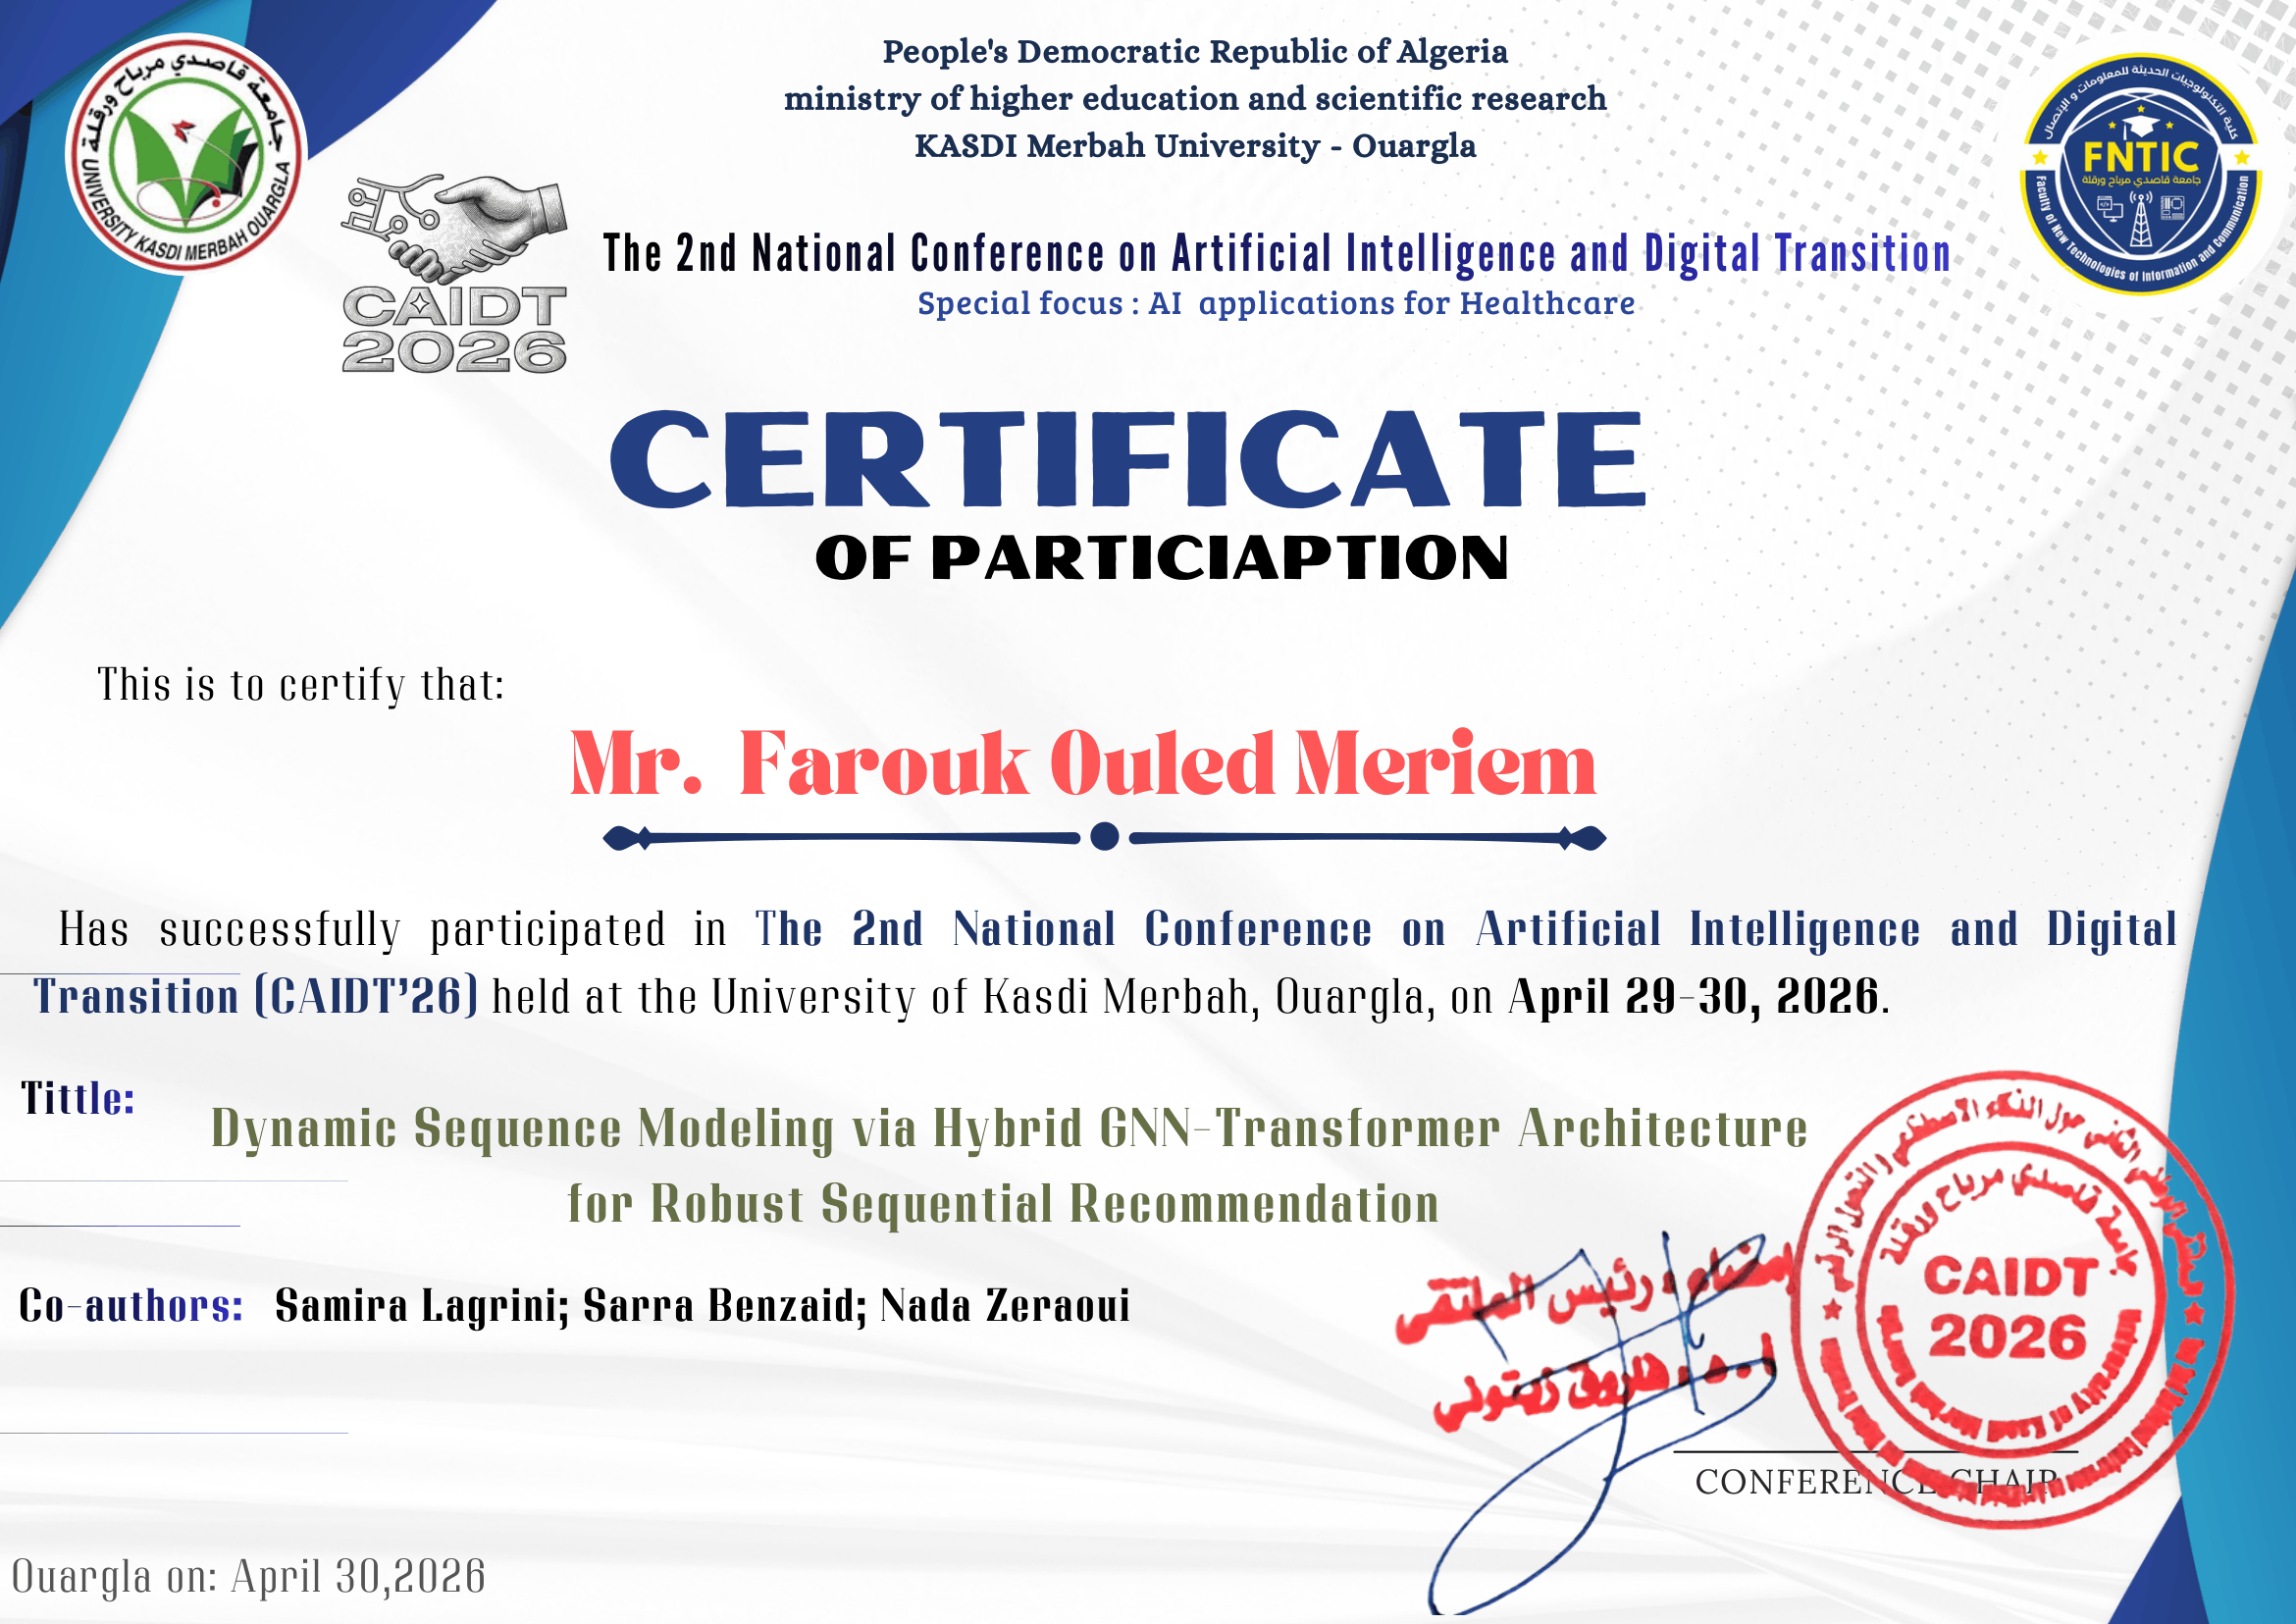
\includegraphics[width=1\textwidth]{picture/certificate of participation.png}
    % CORRECTION: shortened caption to one explicit line
    \caption{Certificate of participation at CAIDT'26, Ouargla, Algeria, April 2026.}
    \label{fig:certificate}
\end{figure}




% ============================================================
%  BIBLIOGRAPHY
% ============================================================
\newpage
\printbibliography[heading=bibintoc, title={References}]

\end{document}